\chapter{Modelling yeast biosynthesis strategies under constraints}
\label{ch:model}

To better understand the mechanistic basis of the YMC, I sought to build a model of how the cyclic sequence of cellular events respond to extracellular nutrient conditions.
However, it is challenging to develop a fine-grained model for the aspects of the YMC,
especially if the detailed molecular mechanisms are unclear.
Further complicating the development of a fine-grained model is the fact that the main read-outs from single-cell studies, NAD(P)H and flavin autofluorescence, are aggregate signals from several biochemical phenomena.
Thus, it is more feasible to construct coarse-grained models to answer biological questions about the YMC.

Here, I use a genome-scale metabolic model and flux balance analysis (FBA) to address whether cellular events in the metabolic cycle reflect a strategy in resource allocation that optimises growth.

Specifically, I aim to evaluate these hypotheses:
\begin{enumerate}
  \item A finite proteome pool gives rise to sequential scheduling of the synthesis of biomass components during growth: lipid, carbohydrate, amino acids, and nucleic acids.
        In other words, as an adaption, the cell synthesises biomass components in sequence rather than in parallel.
        This would explain the timing of biosynthetic events in the phases of the yeast metabolic cycle.
  \item This resource allocation strategy remains advantageous in many nutrient conditions and deletion strains,
        which would explain the robustness of the yeast metabolic cycle.
  \item Synthesis of biomass components in parallel, as opposed to in sequence, may be advantageous if the processes of synthesising each biomass component share similar enzyme levels across biomass components.
\end{enumerate}

\section{Introduction to flux balance analysis}
\label{sec:model-fba}

Metabolic network reconstructions are mathematical representations of a set of metabolic pathways in a living organism.
Usually, each metabolite is represented as a node, and metabolites are connected to each other through reactions that are represented as links \parencite{palssonSystemsBiologyConstraintbased2015}.
This information can be represented in a two-dimensional stoichiometric matrix, in which the rows of the matrix represent the metabolites, the columns represent the reactions, and the values of each element in the matrix show the stoichiometry of the reactions in the system.

For example, if reaction $R_{1}$ is defined by:

\begin{equation}
  \ce{1 M1 + 2 M2 -> 3 M3}
  \label{eq:model-example-chemical-reaction}
\end{equation}

the elements in the stoichiometric matrix that correspond to the metabolite-reaction combinations $(M_{1}, R_{1})$, $(M_{2}, R_{1})$, and $(M_{3}, R_{1})$ are -1, -2, and 3, respectively.

A genome-scale metabolic model is, in simple terms, a metabolic network reconstruction that aims to cover every biochemical reaction in a living system that is catalysed by a gene-encoded enzyme.
In most of the reactions represented in a metabolic network reconstruction, one or more chemical species react to create a different set of chemical species as products.
However, reactions in a metabolic network reconstruction may include processes that are not chemical reactions.
Such processes may include exchange for nutrients, as well as a reaction that models biomass formation.

Flux balance analysis (FBA) is a mathematical method that finds the steady-state flux of reactions through a metabolic network that is best for a given condition \parencite{orthWhatFluxBalance2010}.
These metabolic fluxes represent rates of chemical reactions.
At its core, FBA is a method of solving a linear programming problem of finding the flux values that optimise the output value of an objective function, subject to biological constraints.

Mathematically, the linear programming problem of FBA can be expressed as:

\begin{equation}
  \max \mathbf{c}^{\intercal} \mathbf{v}
  \label{eq:model-fba-objective}
\end{equation}

subject to

\begin{equation}
  \begin{gathered}
    \mathbf{S} \mathbf{v} = \mathbf{0}\\
    v_{i,\mathrm{min}} \leq v_{i} \leq v_{i,\mathrm{max}}
  \end{gathered}
  \label{eq:model-fba-constraints}
\end{equation}

where $\mathbf{c}$ is a vector of weights such that $\mathbf{c}^{\intercal} \mathbf{v}$ defines the objective function, $\mathbf{S}$ is the stoichiometric matrix, and $\mathbf{v}$ is the vector of fluxes. The expression $v_{i,\mathrm{min}}$ the lower bound and $v_{i,\mathrm{max}}$ represents the upper bound for each flux $v_{i}$ in $\mathbf{v}$.

The objective function is given as the task of maximising a mathematical expression that is based on a subset of fluxes (equation~\ref{eq:model-fba-objective}).
Most commonly, the objective function for an FBA problem is maximising the flux of the biomass reaction, thus optimising the growth rate of the cell.
The constraints for FBA are, in the most basic case, imposed by two factors:
the stoichiometric matrix and reaction flux bounds (equation~\ref{eq:model-fba-constraints}).
The stoichiometric matrix balances reaction inputs and outputs, while flux bounds impose upper and lower limits on the fluxes of each reaction.
These constraints restrict the solution space for the FBA problem.

FBA thus offers a computationally inexpensive way to simulate metabolism in a living system, as opposed to solving a large set of differential equations that describe the kinetics of biochemical reactions that are difficult to construct and parametrise.

\section{Modelling temporal scheduling of biosynthesis}
\label{sec:model-temporal}

Previous studies have attempted to use FBA to model how each phase of the YMC has different metabolic requirements.
\textcite{takhaveevTemporalSegregationBiosynthetic2023} showed that in different stages of the cell division cycle, the cell synthesises different components of its biomass at different levels.
In the study, they blocked synthesis of each class of macromolecule and recorded the changes in single-cell NAD(P)H cycles, representing the YMC, to quantify the level of each class of macromolecule that the cell synthesises at each time point within a cell division cycle.
Then, they used these activities as coefficients for a modified thermodynamic-stoichiometric metabolic model at each time point and used FBA to deduce biomass production rates.
% Does not suggest that synthesis of each class of macromolecule excludes all others (which makes sense).
% Rather, this study confirms that timescale of observed synthesis events matches simulations.
% Do I even cite this?  It's so bad.
Additionally, \textcite{cesurGenomeWideAnalysisYeast} constructed a different FBA model for each YMC phase based on transcriptomic and epigenetic data.
They did so using the GIMME algorithm \parencite{beckerContextSpecificMetabolicNetworks2008}, which excludes reactions that correspond to genes that are not expressed at certain time points.
Both studies model the metabolic state of the cell at each phase of the YMC, rather than predicting the time the cell takes to replicate or to synthesise biomass components.

An attempt in extending FBA to solve a time-dependent resource allocation problem was \textcite{reimersCellularTradeoffsOptimal2017}.
This study extended a genome-scale model of the cyanobacterium \textit{Synechococcus elongatus} PCC7942 to find the temporal order of intracellular synthesis reactions which optimises the growth rate of the cell, under resource constraints.
However, the model relies on an external oscillator --- namely, the light-dark cycle.
In contrast, the yeast metabolic cycle is autonomously generated.
Therefore, it is difficult to extend the ideas in \textcite{reimersCellularTradeoffsOptimal2017} to the study of the YMC.

Traditional genome-scale models assume that the uptake rate of carbon source limits production.
However, levels of each enzyme also restrict reaction fluxes, leading to the development of enzyme-constrained models.
An enzyme-constrained model fits the assumption that there is a fixed number of amino acids the cell has to distribute \parencite{weisseMechanisticLinksCellular2015}.
Models like \textcite{sanchezImprovingPhenotypePredictions2017} and \textcite{elsemmanWholecellModelingYeast2022} constrain the total sum of fluxes based on a defined total amount of enzyme.
\textcite{elsemmanWholecellModelingYeast2022} additionally impose a ribosome capacity constraint and additionally imposes compartment constraints.

In this chapter, I used an enzyme-constrained genome-scale model of \textit{Saccharomyces cerevisiae} and performed FBA to simulate temporal scheduling of biomass components.
To simulate the cell prioritising the synthesis of each biomass component, I ablated metabolites from the biomass reaction so that one biomass component remained, then optimised the model.
To assess the advantage of sequential synthesis of biomass components over parallel synthesis of biomass components, I estimated the timescales for the synthesis of each biomass component based on the ablations, and compared them to timescales estimated based on the unmodified biomass reaction.
To evaluate the hypothesis that a restricted proteome pool gives rise to sequential synthesis of biomass components, I varied the size of the proteome pool to observe its effects on the cell's preferred resource allocation strategy.
Finally, to show how nutrient conditions affect the cell's preferred resource allocation strategy, I modelled changes in carbon and nitrogen source concentrations and investigated their effects on the quantities that explain the strategies.

\section{The Yeast8 and ecYeast8 models and their formalisms}
\label{sec:model-yeast8}

To impose proteome constraints, I use the enzyme-constrained Yeast8 (ecYeast8) model \parencite{luConsensusCerevisiaeMetabolic2019} and performed FBA.
I use this model because it is recent, offering a good coverage of reactions, and is continuously updated in a well-characterised and well-documented software repository.
Here, I use the model ec\-Yeast\-8.6.0, the latest version for which both original and enzyme-constrained variants are available.
ecYeast8 uses the GECKO formalism \parencite{sanchezImprovingPhenotypePredictions2017} --- specifically, GECKO 2 \parencite{domenzainReconstructionCatalogueGenomescale2022}, the latest published version of GECKO.
GECKO applies an enzyme constraint by modifying the stoichiometric matrix of a genome-scale metabolic model.
In addition, the model has `pseudometabolites' defined by reactions that group specific chemical species in general classes.
These formalisms allow studying each class of biomass component (e.g. lipid, protein, carbohydrate) individually.

In this section, I discuss the formalisms used in ecYeast8 because they differ from the usual formalisms used in genome-scale metabolic models.

ecYeast8 contains four formalisms relevant to this chapter:
\begin{enumerate}
  \item
        The biomass reaction is defined by having `pseudometabolites' as reactants and a biomass species as a product.
        These pseudometabolites include lipids, proteins, carbohydrates, RNA, DNA, ions, and cofactors.
        This is in contrast to BiGG genome-scale models \parencite{norsigianBiGGModels20202020}.
        In these models, biomass reactions have chemical species as reactants, and each has a stoichiometric coefficient that is equal to the species' abundance in units of \SI{}{\mmolgdw}.
  \item
        The pseudometabolites are defined by `\textit{isa}' reactions, which group specific chemical species into classes of metabolites \parencite{heavnerYeastExpandedReconstruction2012}.
        These reactions account for how some KEGG definitions of reactions require generic compounds and these reactions also allows flexibility of biomass definition in different growth conditions.
        The \textit{isa} reactions have chemical species as reactants, each with a stoichiometric coefficient representing the species' abundance in units of \SI{}{\mmolgdw}, and a pseudometabolite as a product.
        In effect, the species abundance information is shifted one reaction away from the biomass reaction.
  \item
        The models implements SLIMEr \parencite{sanchezSLIMErProbingFlexibility2019}, which Splits Lipids Into Measurable Entities, and adds constraints on lipid classes and acyl chain distribution.
        This formalism is needed because species of lipid backbones and acyl chain can combine to form lipids in more than a thousand ways, and the resulting lipid species are difficult to all be represented in a genome-scale metabolic model.
        SLIMEr thus introduces reactions that split lipids into their basic components and lipid pseudoreactions to preserve the distribution of acyl chains.
        As a result, the definitions of lipids are flexible.
  \item
        GECKO was applied to Yeast8 to produce ecYeast8.  GECKO modifies the stoichiometric matrix of an input genome-scale metabolic model to account for enzyme abundances and kinetics.
        Specifically, it adds to enzyme-catalysed reactions enzyme species with a stoichiometric coefficient derived from its $k_{cat}$ value.
        The formalism also adds reactions to model drawing enzymes from a pool.
        GECKO simulates an upper limit of amino acids available for enzyme production.
\end{enumerate}

Here, I detail how I apply these formalisms for this chapter.
% TODO: Use proper refs rather than hard-coding numbers.
In particular, I detail GECKO (item 4) and computing molecular weights of pseudometabolites (based on items 1 and 2).

% FIXME: Delete this subsection?
% It's mostly a duplicate of the appendix of the GECKO paper,
% and I wrote it just to make sure I understand it.
% I haven't used it in discussion so far.
% FIXME: CHECK FOR PLAGIARISM!!!
\subsection{GECKO}
\label{subsec:model-yeast8-gecko}

\begin{figure}
  \centering
  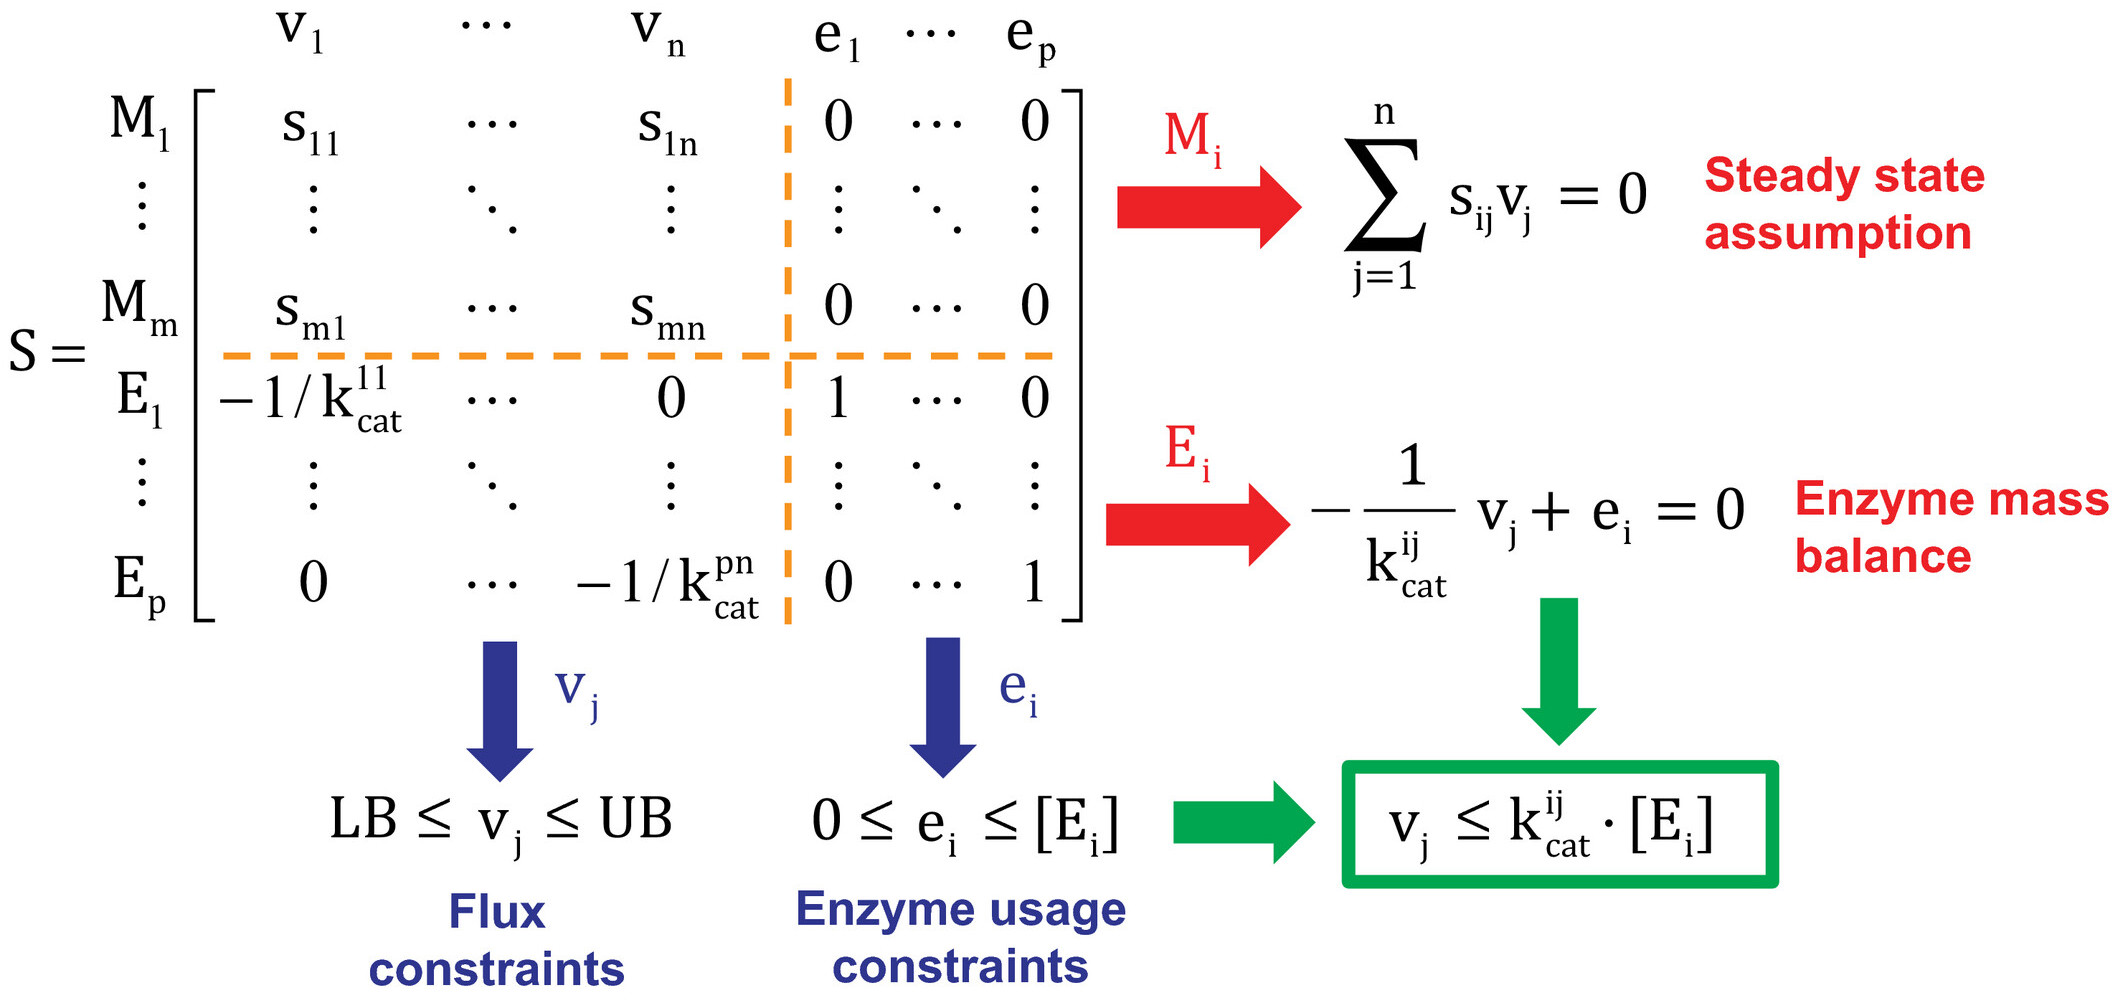
\includegraphics[width=0.9\linewidth]{sanchezImprovingPhenotypePredictions2017_1b_adapted}
  \caption{
    GECKO extends the stoichiometric matrix of a genome-scale model.
    The original stoichiometric matrix $\mathbf{S}$ includes metabolites $M_{1} \ldots M_{m}$ and reactions $v_{1} \ldots v_{n}$.
    GECKO extends this matrix to include enzymes $E_{1} \ldots E_{p}$ and enzyme usage reactions $e_{1} \ldots e_{p}$.
    The new stoichiometric matrix can be seen as four submatrices concatenated together: the upper right submatrix is $\mathbf{0}$, the lower left submatrix encodes kinetic information, and the lower right submatrix is $\mathbf{I}$.
    Figure adapted from~\textcite{sanchezImprovingPhenotypePredictions2017}.
  }
  \label{fig:model-gecko}
\end{figure}

In a conventional genome-scaled model, metabolic fluxes through reactions are constrained by lower and upper bounds.
This constraint narrows down the solution space when the objective function is optimised.
GECKO imposes an additional constraint on the metabolic fluxes based on the concentration of the enzyme that catalyses the reaction (figure~\ref{fig:model-gecko}).

GECKO modifies the linear programming of FBA as defined by equations~\ref{eq:model-fba-objective} and~\ref{eq:model-fba-constraints} so that enzymes are expressed as metabolites that take part in reactions.
In mathematical terms, this can be expressed as:

\begin{equation}
  \max \mathbf{c}^{\intercal} \mathbf{v}
  \label{eq:model-gecko-fba-objective}
\end{equation}

subject to

\begin{equation}
  \begin{gathered}
    \mathbf{S} \mathbf{v} = \mathbf{0}\\
    v_{j,\mathrm{min}} \leq v_{j} \leq v_{j,\mathrm{max}}\\
    v_{j} \leq k_{\mathrm{cat}}^{ij} \cdot [E_{i}]
  \end{gathered}
  \label{eq:model-gecko-fba-constraints}
\end{equation}

where $v_{j}$ is the flux of each reaction $R_{j}$ catalysed by enzyme $E_{i}$, $k_{\mathrm{cat}}^{ij}$ is the catalytic constant of the enzyme $E_{i}$ for reaction $R_{j}$, and $[E_{i}]$ represents the concentration of the enzyme $E_{i}$.
Defining constraints in this way means that each $v_{j}$ must not exceed $v_{\mathrm{max}}$ for each enzyme $E_{i}$.
Each enzyme $E_{i}$ may catalyse one or more reactions $R_{j}$.

The constraints in Eq.\ \ref{eq:model-gecko-fba-constraints} is imposed by extending the stoichiometric matrix $\mathbf{S}$ and flux vector $\mathbf{v}$.
Specifically, $\mathbf{S}$ has additional rows to represent new metabolites that represent each enzyme $E_{i}$.
The matrix $\mathbf{S}$ also has additional columns for new reactions $ER_{i}$ that model enzyme usage and for a new reaction $ER_{\mathrm{pool}}$ that models a limited proteome pool.
Kinetic information in the form of $k_{\mathrm{cat}}^{ij}$ values are included as elements in the extended stoichiometric matrix.
Finally, $\mathbf{v}$ has additional elements that correspond to the additional columns of $\mathbf{S}$.

The constraint $v_{j} \leq k_{\mathrm{cat}}^{ij} \cdot [E_{i}]$ from Eq.\ \ref{eq:model-gecko-fba-constraints} can be expressed as:

\begin{equation}
  \begin{gathered}
    -\frac{1}{k_{\mathrm{cat}}^{ij}}v_{j} + e_{i} = 0\\
    0 \leq e_{i} \leq [E_{i}]
  \end{gathered}
  \label{eq:model-gecko-fba-constraints-extended}
\end{equation}

where $e_{i}$ represents the flux of an enzyme usage reaction $ER_{i}$ associated with $E_{i}$.

To illustrate what the modified stoichiometric means for each reaction, consider a simple example, a reaction $R_{j}$ catalysed by enzyme $E_{i}$:

\begin{equation}
  \ce{ A + B ->[E_{i}] C + D }
  \label{eq:model-gecko-catalysed}
\end{equation}

For this reaction, GECKO imposes (see Eq.\ \ref{eq:model-gecko-fba-constraints}):

\begin{equation}
  v_{j} \leq k_{\mathrm{cat}}^{ij} \cdot [E_{i}]
  \label{eq:model-gecko-kcat}
\end{equation}

where $v_{j}$ is the flux of the reaction $R_{j}$, $k_{\mathrm{cat}}^{ij}$ is the catalytic constant of the enzyme $E_{i}$, and $[E_{i}]$ is the concentration of the enzyme $E_{i}$.

To apply this constraint, GECKO modifies reactions in the genome-scale model.
For example, using Eq.\ \ref{eq:model-gecko-catalysed},
GECKO adds a term to the equation, modifying the stoichiometric matrix, to make it:

\begin{equation}
  \ce{ n_{ij}E_{i} + A + B -> C + D }
  \label{eq:model-gecko-catalysed-formalism}
\end{equation}
with the stoichiometric coefficient $n_{ij} = 1/k_{\mathrm{cat}}^{ij}$.

This transformation, adding the enzyme as a pseudo-reactant, is based on the intuition that the system uses some amount of enzyme at a specific time to catalyse the flux going through the reaction.

Slightly different formalisms are applied to reversible reactions, isozymes, promiscuous enzymes, and enzyme complexes.
Namely:
\begin{itemize}
  \item Reversible reactions are modelled as the forward and reverse reactions separately.
  \item For isozymes, the original reaction is copied multiple times corresponding to the number of reactions that the isozyme catalyses.
        Each has an isozyme catalysing the reaction.
        In addition, there is an `arm' reaction to act as an intermediate between the substrate and the products.
  \item No actions are needed for promiscuous enzymes.
  \item Enzyme complexes are modelled as one reaction that uses all subunit proteins that all share the same $k_{cat}$ value.
\end{itemize}

GECKO adds an enzyme as a pseudo-reactant for all enzyme-catalysed reactions in the genome-scale model to create an enzyme-constrained model.

To constrain enzyme levels in the model, GECKO defines a pseudo-reaction

\begin{equation}
  ER_{\mathrm{pool}}: \varnothing \ce{ -> E_{pool} }
  \label{eq:model-gecko-enzyme-pool}
\end{equation}

with a flux

\begin{equation}
  \epool \leq (P_{\mathrm{total}} - P_{\mathrm{measured}}) \cdot f \cdot \sigma
  \label{eq:model-gecko-enzyme-pool-flux}
\end{equation}

in units of \SI{}{\gram~\gram_{DW}^{-1}}, where

\begin{itemize}
  \item $P_{\mathrm{total}}$ is the total protein fraction with respect to the dry weight of the cell
  \item $P_{\mathrm{measured}}$ is the protein fraction of proteins whose weight are accounted for in the model, based on proteomic data.
        If no proteomic data is used, as is the case in this chapter, $P_{\mathrm{measured}} = 0$.
  \item $f$ represents the fraction of proteins that are enzymes
  \item $\sigma$ is a parameter that represents the average saturation of enzymes
\end{itemize}

ecYeast8.6.0 assumes parameter values of: $f = 0.5$, $P_{\mathrm{total}} = 0.5$, and $\sigma = 0.5$.

Defining such parameters is a judgement call, especially when the protein fraction varies across growth rates~\parencite{elsemmanWholecellModelingYeast2022}, but $f = 0.5$ is close to the protein mass fraction of ecYeast8.6.0 (to be discussed in section~\ref{subsec:model-yeast8-molweights}).
Subsequently, GECKO changes the carbohydrate composition based on the assumption that a change in the amino acid composition is offset by the reverse change in the carbohydrate composition;
experimental data justifies this assumption \parencite{nissenFluxDistributionsAnaerobic1997}.

Then, for each enzyme $\ce{E_{i}}$, GECKO defines enzyme usage pseudoreactions of the form

\begin{equation}
  ER_{i}: \ce{ MW_{i} E_{\mathrm{pool}} -> E_{i} }
  \label{eq:model-gecko-enzyme-usage}
\end{equation}

with $\mathrm{MW}_{i}$ being the molecular weight of the enzyme in units of \SI{}{\gram~\milli\mole^{-1}}.
The flux of enzyme usage pseudoreactions are defined in units of \SI{}{\mmolgdw}.

Taken together, the modelled cell thus has an enzyme pool in terms of a mass fraction of the cell's dry weight, and the modelled cell allocates certain fractions of this mass to the synthesis of each enzyme at steady-state.  The mass of each enzyme in the cell determines the amount (in moles) of each enzyme and therefore its catalytic activity.

GECKO takes $k_{cat}$ values from BRENDA \parencite{changBRENDAELIXIRCore2021} and enzyme data from SWISSPROT \parencite{theuniprotconsortiumUniProtUniversalProtein2023} and KEGG \parencite{kanehisaKEGGTaxonomybasedAnalysis2023}, including molecular weight of proteins and associated pathways.

\subsection{Computing molecular weights of pseudometabolites}
\label{subsec:model-yeast8-molweights}

To compute the time it takes for the yeast cell to synthesise each biomass component, the mass fractions of each biomass component must be known.
%In the yeast cell, biomass components (lipids, carbohydrates, proteins) are present in different fractions.
%Knowing these fractions is useful in computing the time it takes to synthesise each biomass component.
In genome-scale metabolic models, these mass fractions are represented in the biomass reaction, set as the objective function, which is defined as:

\begin{equation}
  \ce{f_{1}M1 + f_{2}M2 + ... + f_{n}M_{n} -> B}
  \label{eq:model-biomass-reaction}
\end{equation}

where $M_{1} \ldots M_{n}$ represent the chemical species that make up the cell's biomass, the stoichiometric coefficients $f_{1} \ldots f_{n}$ represent the mass fraction of each species in units of \SI{}{\gram~\gram_{DW}^{-1}}, and $B$ represents biomass.
If a chemical species $M_{i}$ has a mass fraction $f_{i}$, then \SI{1}{\gram} of cell dry weight has $f_{i}$ \SI{}{\gram} of chemical species $M_{i}$.

However, the mass fraction of each biomass component varies according to strain and growth rate \parencite{nilssonMetabolicTradeoffsYeast2016, elsemmanWholecellModelingYeast2022}.
It is not straightforward to implement these changes as stoichiometric coefficients of the chemical species that define biomass, because there is limited information for the mass fractions of such species as conditions vary, and because of the many combinations of lipid backbones and acyl chains.

Therefore, I computed the mass fractions of each biomass component based on the stoichiometries of species in the Yeast8 model.%, as a back-of-the-envelope calculation for such a coarse-grained modelling effort.
%Similar calculations were performed by \textcite{takhaveevTemporalSegregationBiosynthetic2023}.
This is not as straightforward as taking the $f_{i}$ values from an objective function defined as in Eq.\ \ref{eq:model-biomass-reaction}, because the objective function of Yeast8 does not conform to this format, and instead contains pseudometabolites.
This formalism can be expressed as:

\begin{equation}
  \begin{aligned}
    \ce{f_{1}M_{B,1} + ... + f_{n}M_{B,n} + f_{n+1}P1 + ... + f_{n+k}P_{k} &-> B}\\
    \ce{f_{P_{1},1}M_{P_{1},1} + ... + f_{P_{1},n}M_{P_{1},n} &-> P1}\\
    &\ldots\\
    \ce{f_{P_{k},1}M_{P_{k},1} + ... + f_{P_{k},n}M_{P_{k},n} &-> P_{k}}
    \label{eq:model-pseudometabolites}
  \end{aligned}
\end{equation}

where each $M$ is a chemical species with a defined molecular weight, each $P$ is a pseudometabolite, and each $f$ is a stoichiometric coefficient.
The objective function remains the reaction that produces $B$, but some chemical species $M_{B,1} \ldots M_{B,n}$ are retained in the objective function, while other chemical species are replaced by pseudometabolites $P_{1} \ldots P_{k}$.
The reactions that produce $P_{1} \ldots P_{k}$ are \textit{isa} reactions.
\textit{isa} reactions define pseudometabolites by having chemical species with known molecular weights as reactants, with their stoichiometric coefficients representing abundance in \SI{}{\mmolgdw}.
In Yeast8, the objective function is defined as:

\texttt{
  47.5883 atp\_c + 47.5883 h2o\_c + lipid\_c + protein\_c + carbohydrate\_c\\
  + dna\_c + rna\_c + cofactor + ion \\
  --> 47.5883 adp\_c + biomass\_c + 47.5883 h\_c + 47.5883 pi\_c
}

Here, there are seven pseudometabolites: lipid, protein, carbohydrate, DNA, RNA, cofactor, and ion.

As the ecYeast8 model does not specify the molecular weights of these pseudometabolites, in order to obtain the mass fraction of each biomass component represented by the pseudometabolites,
I treated each pseudometabolite as a chemical species and calculated its molecular weight by assuming mass balance \parencite{chanStandardizingBiomassReactions2017, dinhQuantifyingPropagationParametric2022, takhaveevTemporalSegregationBiosynthetic2023}.
Namely, I assumed that in reactions that produce the pseudometabolites, there is conservation of mass, and therefore:

% To this end, I first computed molecular weights for pseudometabolites that represent macromolecules and other biomass components in the ecYeast8 model, as
% the ecYeast8 model does not specify the molecular weights of these pseudometabolites.
% The pseudometabolites include: lipids, proteins, carbohydrates, RNA, DNA, cofactors, and ions.
% Namely, I assumed that in reactions that produce the pseudometabolites, there is conservation of mass, and therefore:

\begin{equation}
  \sum_{r = j}^{n_{r}}m_{r}c_{r} = \sum_{p = i}^{n_{p}}m_{p}c_{p}
\label{eq:conservation-of-mass}
\end{equation}

where
$s = 1, \ldots n_{s}$ represents substrates of the reaction in question,
$p = 1, \ldots n_{p}$ represents products.
$m_{r}$ represents molar mass of reactant $r$,
$m_{p}$ represents molar mass of product $p$,
$c_{r}$ represents stoichiometric coefficient of reactant $r$, and
$c_{p}$ represents stoichiometric coefficient of product $p$.

The resulting molecular weight will thus represent the mass fraction of each biomass component in units of \SI{}{\gram~\gram_{DW}^{-1}}.


\subsubsection{Carbohydrate, DNA, RNA, cofactor, and ion pseudometabolites}
\label{subsubsec:model-yeast8-molweight-easy}

Computing the molecular weights of the carbohydrate, DNA, RNA, cofactor, and ion pseudometabolites is straightforward.
This is because the equations similarly have reactants with molecular weights specified in the model and only the pseudometabolite, the sole product, does not have a molecular weight specified.
In such cases, Eq.\ \ref{eq:conservation-of-mass} can be applied directly, i.e.\ the molecular weight of the pseudometabolite is equal to $\sum_{r = j}^{n_{r}}m_{r}c_{r}$, where $m_{r}$ values are taken directly from the molecular weights specified in the model.
The results for these pseudometabolites are shown in table~\ref{tab:ecyeast8-easy-rxns}

\begin{table}[ht]
  \centering
    \begin{tabular}{llS}
      ID & Reaction & {\makecell{Computed molecular\\ weight (\SI{}{\gram~\mole^{-1}})}} \\
      \hline
      \texttt{r\_4048} & \makecell{\texttt{0.684535 (1->3)-beta-D-glucan} \\ \texttt{ + 0.228715 (1->6)-beta-D-glucan} \\ \texttt{+ 0.330522 glycogen + 0.650171 mannan} \\ \texttt{ + 0.126456 trehalose} \\ \texttt{--> carbohydrate}} & 350.37 \\
    \texttt{r\_4050} & \makecell{\texttt{0.0036 dAMP + 0.0024 dCMP + 0.0024 dGMP} \\ \texttt{ + 0.0036 dTMP} \\ \texttt{--> DNA}} & 3.90 \\
    \texttt{r\_4049} & \makecell{\texttt{0.0445348 AMP + 0.0432762 CMP} \\ \texttt{+ 0.0445348 GMP + 0.0579921 UMP} \\ \texttt{--> RNA}} & 64.04 \\
    \texttt{r\_4598} & \makecell{\texttt{0.00019 coenzyme A + 1e-05 FAD} \\ \texttt{ + 0.00265 NAD + 0.00015 NADH} \\ \texttt{ + 0.00057 NADP(+) + 0.0027 NADPH} \\ \texttt{ + 0.00099 riboflavin + 1.2e-06 TDP} \\ \texttt{ + 6.34e-05 THF + 1e-06 heme a} \\ \texttt{--> cofactor}} & 4.83 \\    \texttt{r\_4599} & \makecell{\texttt{3.04e-05 iron(2+) + 0.00363 potassium} \\ \texttt{ + 0.00397 sodium + 0.02 sulphate} \\ \texttt{ + 0.00129 chloride + 0.00273 Mn(2+)} \\ \texttt{ + 0.000748 Zn(2+) + 0.000217 Ca(2+)} \\ \texttt{ + 0.00124254 Mg(2+) + 0.000659 Cu(2+)} \\ \texttt{--> ion}} & 2.48 \\
    \end{tabular}
    \caption{Straightforward cases of computing pseudometabolite molecular weights from pseudoreactions in ecYeast8}
    \label{tab:ecyeast8-easy-rxns}
\end{table}


\subsubsection{Protein pseudometabolite}
\label{subsubsec:model-yeast8-molweight-protein}

Other metabolites were less straightforward and required some judgement calls.
To compute the molecular weight of the protein pseudometabolite, I inspected reaction \texttt{r\_4047}:

\texttt{
  0.57284 Ala-tRNA(Ala) + 0.200644 Arg-tRNA(Arg) + 0.126979 Asn-tRNA(Asn)\\
  + ... + 0.330369 Val-tRNA(Val) \\
  --> 0.57284 tRNA(Ala) + 0.200644 tRNA(Arg) + 0.126979 tRNA(Asn) \\
  + ... + 0.330369 tRNA(Val) + protein
}

In Yeast8, aminoacyl-tRNA and tRNA species do not have molecular weights specified in the model.
This is because their chemical formulas are incompletely specified in the model as the model uses \texttt{R} to represent the tRNA.
For example, \texttt{Ala-tRNA(Ala)}, alanyl-tRNA, is represented as \texttt{C3H7NOR}, and \texttt{tRNA(Ala)} is represented as \texttt{RH}.
As a consequence, the molecular weights of these species cannot be directly computed from the chemical formula.
Because tRNAs are unmodified during translation, \texttt{R} can be ignored.
In other words, I treated \texttt{R} as a chemical element of atomic mass 0 when computing $m_{r}$ for each reactant and $m_{p}$ for each product, leaving only $m_{p}$ for \texttt{protein} undefined.
This $m_{p}$ can then be found by rearranging Eq.\ \ref{eq:conservation-of-mass}, thus giving the molecular mass of the protein pseudometabolite.


\subsubsection{Lipid pseudometabolite}
\label{subsubsec:model-yeast8-molweight-lipid}

Finally, the lipid pseudometabolite is the least straightforward because the model does not specifiy the molecular weights of some of the reactants of the lipid pseudoreaction.
The lipid pseudoreaction is represented in reaction \texttt{r\_2108}:

\texttt{
  lipid backbone + lipid chain --> lipid
}

And both \texttt{lipid backbone} and \texttt{lipid chain} have no molecular weight specified.

Reaction \texttt{r\_4065} specifies a lipid chain pseudoreaction, in which \texttt{lipid chain} is generated:

\texttt{
  0.0073947 C16:0 chain + 0.0217019 C16:1 chain + 0.0020726 C18:0 chain \\
  + 0.000796243 C18:1 chain \\
  --> lipid chain
}

As all reactants have molecular weights defined in the model, the molecular weight of \texttt{lipid chain} can be computed from the mass balance of this reaction.

Reaction \texttt{r\_4063} specifies a lipid backbone pseudoreaction, in which \texttt{lipid backbone} is generated:

\texttt{
  0.000631964 1-phosphatidyl-1D-myo-inositol backbone\\
  + 0.00243107 ergosterol + 0.000622407 ergosterol ester backbone\\
  + 0.000135359 fatty acid backbone + ...\\
  --> lipid backbone
}


\begin{table}[ht]
  \centering
    \begin{tabular}{llS}
      ID & Reaction & {\makecell{Computed molecular\\ weight (\SI{}{\gram~\mole^{-1}})}} \\
      \hline
    \texttt{r\_3975} & \makecell{\texttt{palmitate} \\ \texttt{--> 0.255421 fatty acid backbone} \\ \texttt{0.256429 C16:0 chain}} & 742.54 \\
    \texttt{r\_3976} & \makecell{\texttt{palmitoleate} \\ \texttt{--> 0.253405 fatty acid backbone} \\ \texttt{0.254413 C16:1 chain}} & 744.56 \\
    \texttt{r\_3977} & \makecell{\texttt{stearate} \\ \texttt{--> 0.283475 fatty acid backbone} \\ \texttt{0.284483 C18:0 chain}} & 714.49 \\
    \texttt{r\_3978} & \makecell{\texttt{oleate} \\ \texttt{--> 0.281459 fatty acid backbone} \\ \texttt{0.282467 C18:1 chain}} & 716.51 \\
    \end{tabular}
    \caption{ecYeast8 reactions that generate the \texttt{fatty acid backbone} metabolite}
    \label{tab:ecyeast8-fatty-acid-backbone-rxns}
\end{table}

% TODO: Probably needs even more clarification
The model specifies molecular weights for all species in the reaction that generates \texttt{lipid backbone}, expect for \texttt{fatty acid backbone}.
To compute the molecular weight of \texttt{fatty acid backbone}, the reactions that produce this species must be used.
Because of SLIMEr, four reactions in the model produce \texttt{fatty acid backbone} (table~\ref{tab:ecyeast8-fatty-acid-backbone-rxns}).
The model specifies molecular weights for all species in these four reactions, except for \texttt{fatty acid backbone}.
Therefore, using each chemical equation, the molecular weight of \texttt{fatty acid backbone} can be solved for by rearranging Eq.\ \ref{eq:conservation-of-mass} with parameters defined to match each reaction.
However, the molecular weights computed from each equation are different.% , as shown in table~\ref{tab:ecyeast8-fatty-acid-backbone-rxns}.
Because the differences are slight, %, and ultimately I am making a back-of-the-envelope calculation,
I took the mean of the four weights to give \SI{729.53}{\gram~\mole^{-1}}.
Subsequently, the molecular weight of \texttt{lipid backbone} was computed from this mean value and the molecular weights of other species involved in the production of \texttt{lipid backbone}, giving \SI{21.31}{\gram~\mole^{-1}}.
With the molecular weights of \texttt{lipid backbone} and \texttt{lipid chain} defined, the molecular weight of \texttt{lipid} is thus the sum of the two.


\subsubsection{Summary}
\label{subsubsec:model-yeast8-molweight-summary}

\begin{table}[ht]
  \centering
  \begin{tabular}{lSS}
    Metabolite & {\makecell{Computed molecular weight\\ (\SI{}{\gram~\mol^{-1}})}} & {\makecell{Biomass composition\\ at growth rate \SI{0.375}{\hour^{-1}}\\ (\SI{}{\gram~\kilo\gram_{DW}^{-1}})}} \\
    \hline
    Protein & 504.37 & 505.\\
    Carbohydrate & 350.37 & 237.\\
    RNA & 64.04 & 105.\\
    Lipid & 31.57 & 57.\\
    Cofactors & 4.83 & \\
    DNA & 3.90 & 5. \\
    Ions & 2.48 & \\
    \hline
    Total & 961.57 & \\
  \end{tabular}
  \caption{
    Computed molecular weights of bulk metabolites in ecYeast8, compared to experimentally recorded biomass composition by \textcite{canelasVivoDatadrivenFramework2011}.
  }
  \label{tab:ecyeast8-mol-weights}
\end{table}

Table~\ref{tab:ecyeast8-mol-weights} summarises the molecular weight of the pseudometabolites.
As validation of the calculations of molecular weights, the ratio between the molecular weights are similar to the ratio between the mass of each class of macromolecule in the yeast cell dry weight shown by \textcite{canelasVivoDatadrivenFramework2011}.

Adding together values in table~\ref{tab:ecyeast8-fatty-acid-backbone-rxns} gives a  molecular weight of the biomass pseudometabolite of \SI{961.57}{\gram~\mol^{-1}}, close to the \SI{966}{\gram~\mol^{-1}} computed by \textcite{takhaveevTemporalSegregationBiosynthetic2023} from a different genome-scale model.
In theory, this number should be \SI{1000}{\gram~\mol^{-1}} because the stoichiometric coefficients of the species that form biomass components are expressed in terms of \SI{}{\mmolgdw} \parencite{thieleProtocolGeneratingHighquality2010, palssonSystemsBiologyConstraintbased2015}, but the deviation from 1000 could be explained by the SLIMEr formalism.
Plus, the sum of stoichiometric coefficients are not always verified in genome-scale models \parencite{chanStandardizingBiomassReactions2017}.


\section{Ablating pseudometabolites from the biomass reaction}
\label{sec:model-yeast8-pseudometabolites}

\subsection{Definition of ablation}
\label{sec:model-yeast8-pseudometabolites-def}

To simulate producing each class of biomass component in turn,
I take advantage of pseudometabolites in ecYeast8 to remove each of them in turn from the biomass reaction ---
in other words, ablating pseudometabolites from the biomass reaction.
Specifically, I exclude each pseudometabolite from the biomass reaction, in turn, and optimise the model.

Consider the objective function, the biomass reaction:

\texttt{
  47.5883 atp\_c + 47.5883 h2o\_c + lipid\_c + protein\_c + carbohydrate\_c\\
  + dna\_c + rna\_c + cofactor + ion \\
  --> 47.5883 adp\_c + biomass\_c + 47.5883 h\_c + 47.5883 pi\_c
}

There are seven pseudometabolites: lipid, protein, carbohydrate, DNA, RNA, cofactor, and ion.

To have the cell prioritise biosynthesis of lipids, I set the stoichiometric coefficients of all pseudometabolites except for lipids to zero in the above equation, giving:

\texttt{
  47.5883 atp\_c + 47.5883 h2o\_c + lipid\_c \\
  --> 47.5883 adp\_c + biomass\_c + 47.5883 h\_c + 47.5883 pi\_c
}

The model was optimised using FBA, with the modified reaction as the objective function.
This process was repeated for the other pseudometabolites.

\begin{figure}
  \centering
  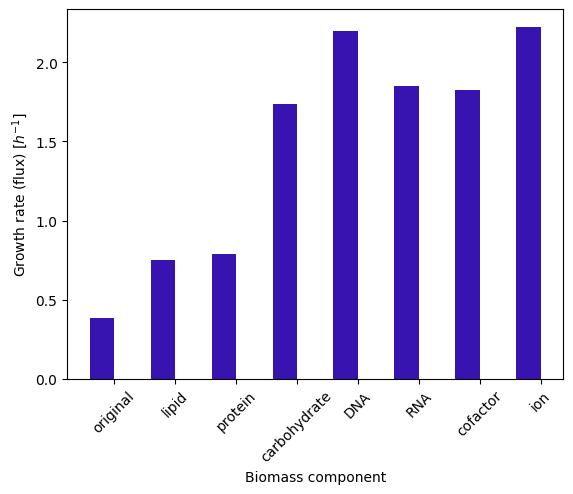
\includegraphics[width=.6\linewidth]{ablation_example_fluxes.png}
  \caption{
    %Growth rates from the original model ($\gro$; leftmost bar) and from the ablated versions of the model ($\griabl$, where $i$ represents each biomass components among lipids, proteins, carbohydrates, DNA, RNA, cofactors, and ions; other bars)
    Growth rates from the original model (leftmost bar) and from the ablated versions of the model (other bars)
  }
  \label{fig:model-ablate-fluxes}
\end{figure}


\subsection{Effect on allocation of proteome}
\label{sec:model-yeast8-pseudometabolites-allocation}

To evaluate whether ablation leads to changes of model behaviour that reflect cellular biochemistry, I quantified how proteome allocation to enzymes changes across rounds of ablation.
When the model prioritises a different biomass component in each round of ablation, the model partitions the limited proteome available for enzyme production differently.
In other words, in each round of ablation, the vector of fluxes carried by each enzyme usage pseudoreaction (defined in Eq.\ \ref{eq:model-gecko-enzyme-usage}) is different from each other and from the non-ablated case, in which all biomass components are synthesised in parallel.
Optimising the objective function as each pseudometabolite is prioritised affects the predicted growth rates (Fig.\ \ref{fig:model-ablate-fluxes}).

Subsystem information aids interpretation of these changes.
Here, I match the flux carried by each enzyme usage pseudoreaction to the enzyme-catalysed reaction that the enzyme is associated with.
If an enzyme usage pseudoreaction is associated with multiple enzyme-catalysed reactions, data entries were duplicated accordingly.
Then, the subsystem associated with each enzyme-catalysed reaction is taken from the gene-protein map, and noted.

To quantify changes in proteome allocation across rounds of ablation, I compute the $\log_{2}(\mathrm{FC})$ of fluxes relative to the non-ablated, parallel case.
This is defined as:

\begin{equation}
  \log_{2}(\mathrm{FC}_{i,j}) = \log_{2}\left( \frac{e_{i,j}^{\prime}}{e_{i, \mathrm{par}}^{\prime}} \right)
  \label{eq:model-foldchange}
\end{equation}

where, to ensure that $\log_{2}(\mathrm{FC}_{i,j})$ can be defined for all $i$ and $j$,

\begin{equation}
  e^{\prime} =
  \begin{cases}
    \epsilon, & \text{if}\ |e|<\epsilon \\
    e, & \text{otherwise}
  \end{cases}
  \label{eq:model-epsilon-round}
\end{equation}

where $e$ is either $e_{i,j}$ or $e_{i, \mathrm{par}}$.
Here, $e_{i, \mathrm{par}}$ represents the flux of an enzyme usage reaction associated with each enzyme $E_{i}$ in the model (defined in Eq.\ \ref{eq:model-gecko-fba-constraints-extended}) in the non-ablated, parallel case, and $e_{i,j}$ represents the flux of the enzyme usage reaction when biomass component $j$ is prioritised in a round of ablation.

The value $\epsilon$ is defined as:

\begin{equation}
  \begin{aligned}
    \epsilon &= \SI{1}{\molecule~\cell^{-1}~\hour^{-1}}\\
             &= \frac{(\SI{1}{\molecule})}{(\SI{1}{\cell})(\SI{1}{\hour})} \cdot \frac{(\SI{1}{\cell})}{(\SI{15}{\pico\gram_{DW}})} \cdot \frac{(\SI{1}{\mol})}{(\SI{6.02214d23}{\molecule)}}\\
             &= \SI{1.11d-13}{\mol~\gram_{DW}^{-1}~\hour^{-1}}\\
             &= \SI{1.11d-10}{\mmolgdwh}\\
  \end{aligned}
  \label{eq:model-epsilon}
\end{equation}

assuming a reasonable minimum reaction flux of \SI{1}{\molecule~\cell^{-1}~\hour^{-1}} and a cell dry weight of \SI{15}{\pico\gram} dry weight per cell \parencite{shermanGettingStartedYeast2002}.

If $\log_{2}(\mathrm{FC_{i,j}}) > 0$, this indicates that the cell allocates more of its proteome to produce enzyme $E_{i}$ when biomass component $j$ is prioritised.
Conversely, if $\log_{2}(\mathrm{FC_{i,j}}) < 0$, the cell allocates less of its proteome to produce enzyme $E_{i}$ when biomass component $j$ is prioritised.
In addition, if there is a case of enzyme expression switching on, evidenced by $e_{i, \mathrm{par}} = 0$, $\log_{2}(\mathrm{FC}_{i,j}) \ll 0$.
Conversely, if there is a case of an enzyme expression switching off, evidenced by $e_{i, j} = 0$, $e_{i,j}$ $\log_{2}(\mathrm{FC}_{i,j}) \gg 0$.

\begin{figure}
  \centering
  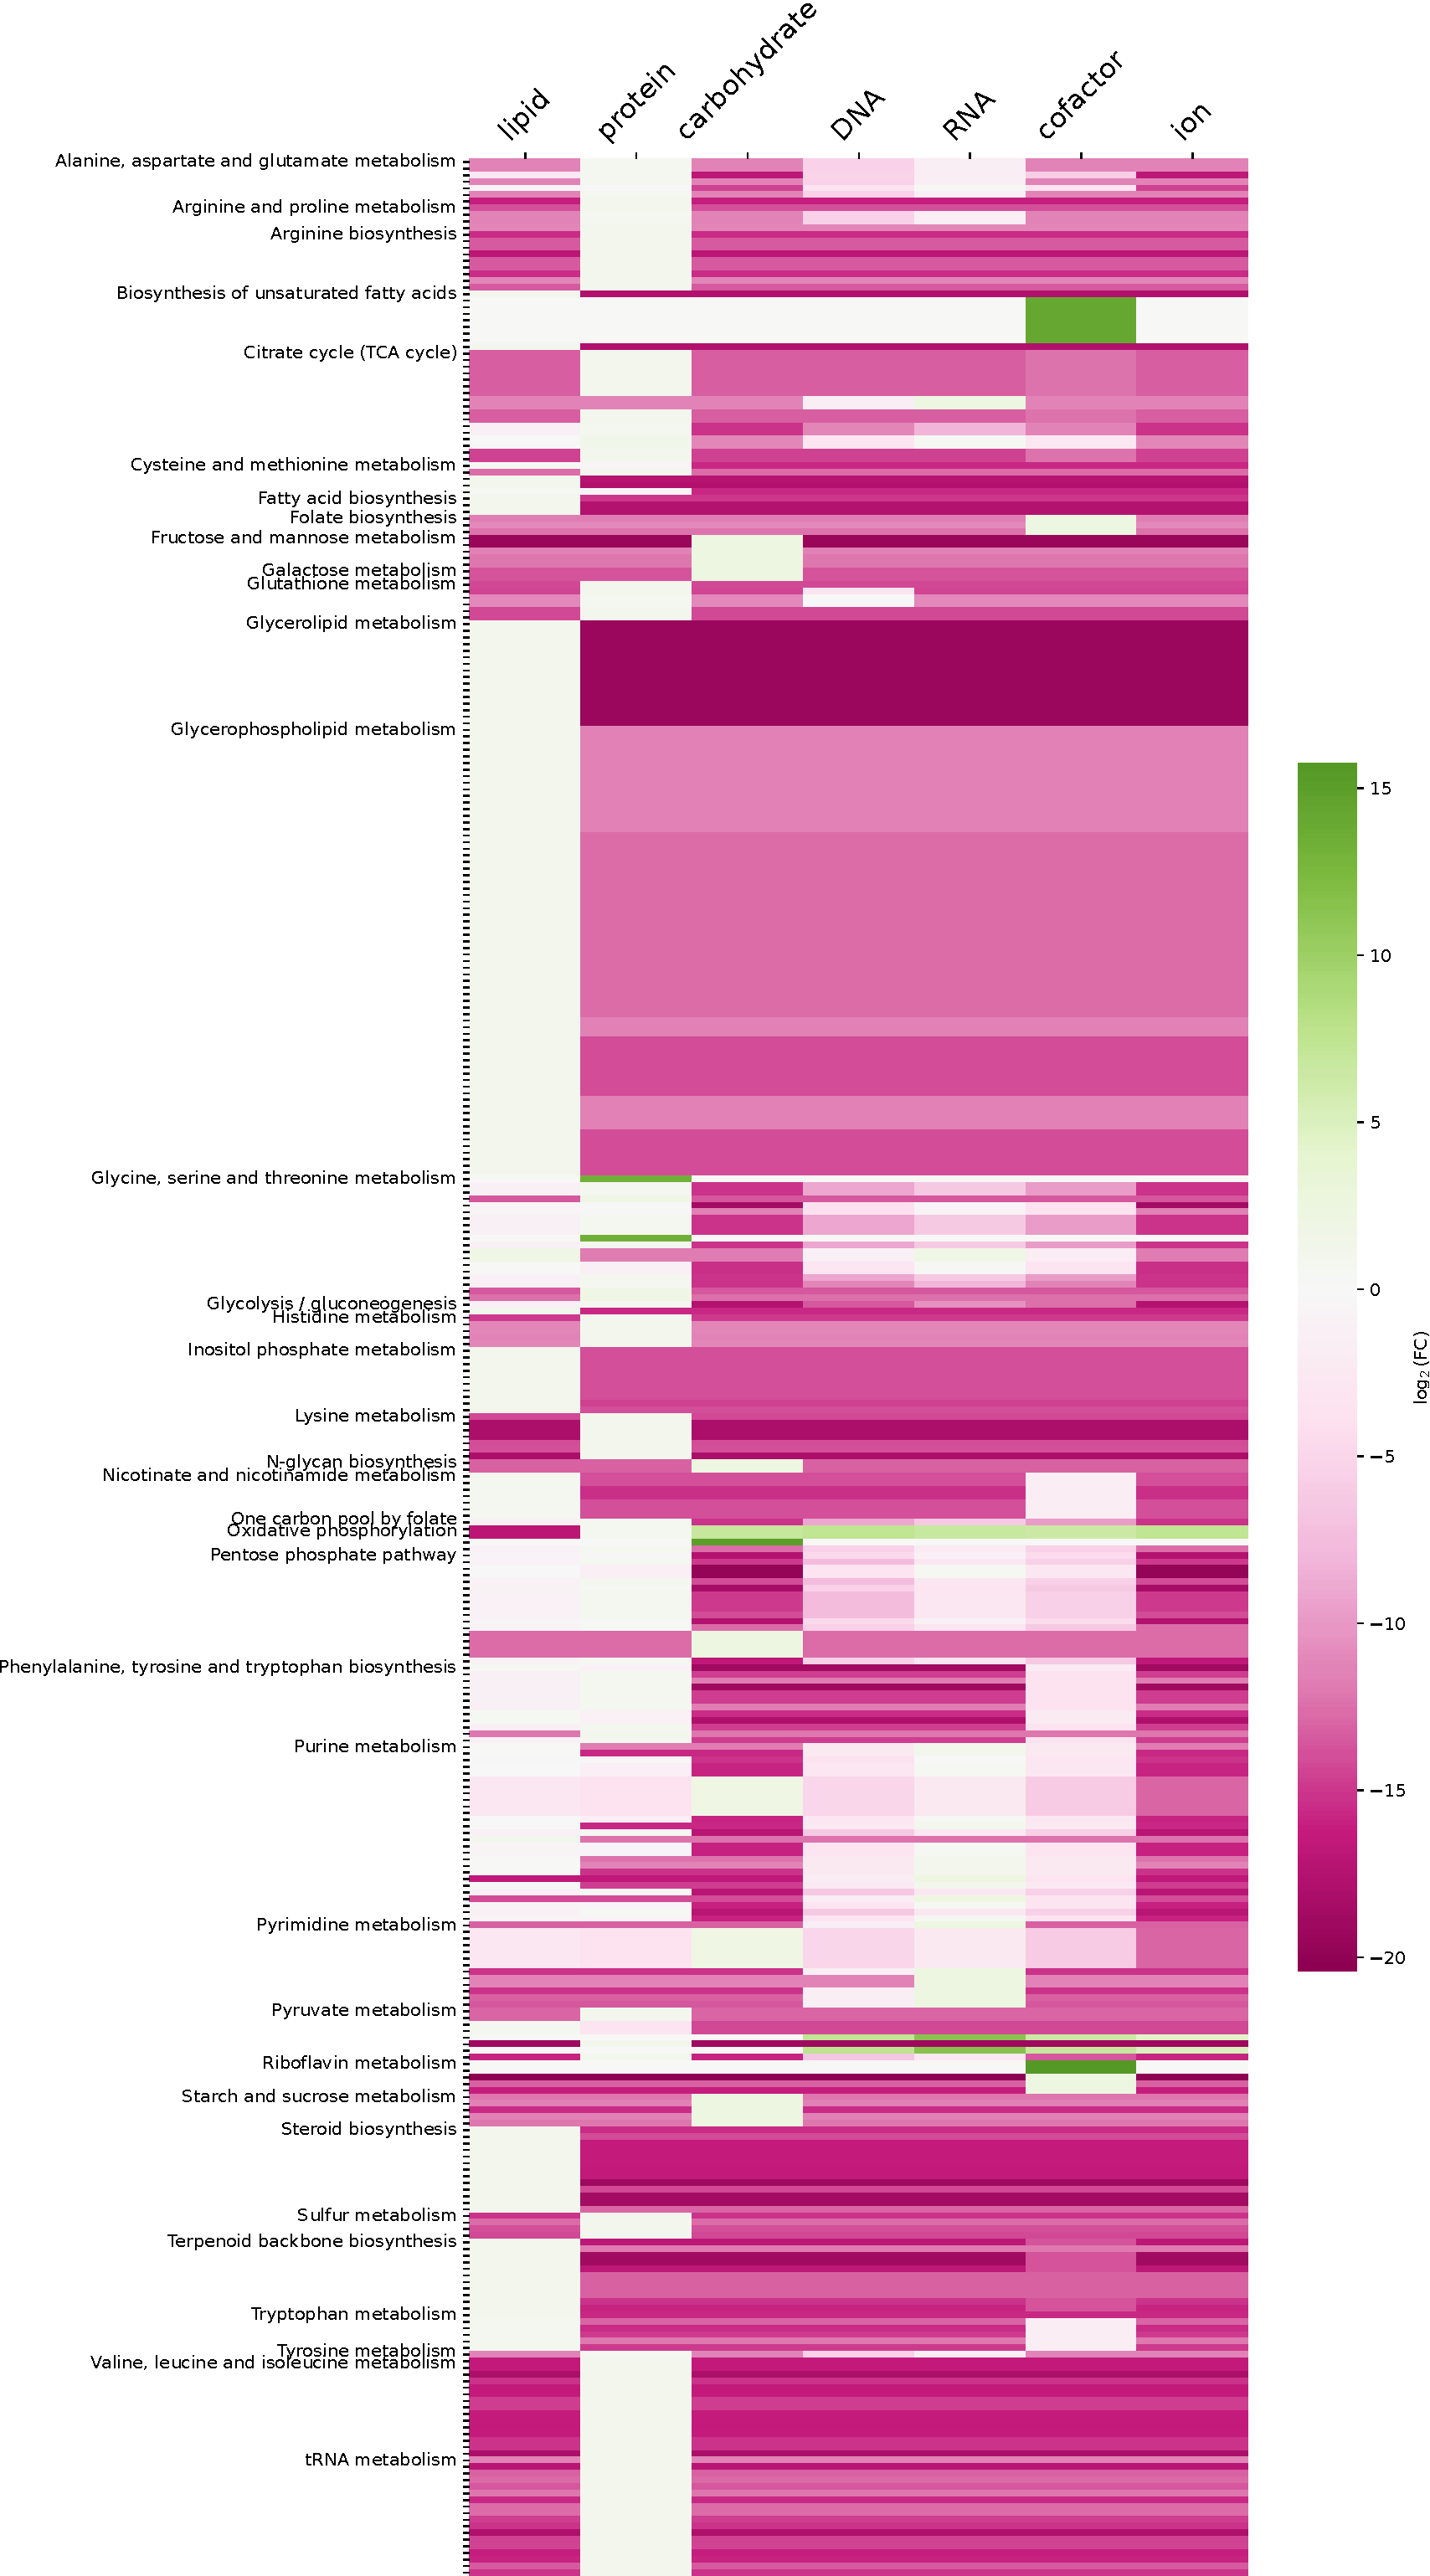
\includegraphics[width=.8\linewidth]{allocation_fc}
  \caption{
    $\log_{2}(\mathrm{FC})$ of enzyme usage reaction flux (Eq.\ \ref{eq:model-gecko-enzyme-usage}) in rounds of ablation, according to biomass component prioritised.
    %The cell changes how it allocates its proteome to enzymes when different components of its biomass are prioritised.
    Each column shows the component that remains in each round of pseudometabolite ablation (labels on top).
    Each row represents an enzyme, and rows are grouped by subsystem (labels on left).
    Colours represent $\log_{2}(\mathrm{FC})$ (Eq.\ \ref{eq:model-foldchange}) showing how enzyme usage fluxes change in rounds of ablation: green shows an increase, while pink shows a decrease.
    Rows in which $|\log_{2}(\mathrm{FC})| < 11$ for all biomass components are excluded to restrict the number of reactions ($n = \num{3897}$) for visualisation.
  }
  \label{fig:model-ablate-enz-use}
\end{figure}

Figure~\ref{fig:model-ablate-enz-use} shows the subsystems and fold changes calculated as described above.
In particular, it shows:

\begin{enumerate}
  \item When any particular biomass component is prioritised, the cell de-allocates its proteome to most of its enzymes, as evidenced by $\log_{2}(\mathrm{FC}_{i,j}) < 0$ for most values of $i, j$.
        However, there are cases in which there are strong increases in allocation, as shown by $\log_{2}(\mathrm{FC}_{i,j}) > 0$.
        For example, when cofactors are prioritised, there are strong increases in biosynthesis of unsaturated fatty acids and in riboflavin metabolism.
        Additionally, there are strong increases in oxidative phosphorylation when carbohydrate, DNA, RNA, cofactor, or ion is prioritised.
  \item When the cell prioritises lipid biosynthesis, it exhibits the least change relative to the parallel (non-ablated case), compared to cases in which other biomass components are prioritised.
        The changes include increases of fluxes in the subsystems of fatty acid biosynthesis, glycerolipid metabolism, glycerophospholipid metabolism, inositol phosphate metabolism, steroid biosynthesis, and terpenoid backbone.
        Given that these subsystems are directly related to lipid metabolism, such changes are expected.
        In addition, during lipid biosynthesis, the model shows decreases of fluxes in oxidative phosphorylation, the TCA cycle, and in amino acid metabolism, with fluxes varying depending on the amino acid.
  \item When the cell prioritises protein biosynthesis, it shows small increases in fluxes associated with amino acid metabolism, tRNA metabolism, and oxidative phosphorylation.
        Such increases are expected as these led to production of substrates that are required for translation.
        Conversely, when other biomass components (carbohydrate, ion, DNA, RNA, and cofactor) are prioritised, there are decreases in fluxes in glycine, serine, and threonine metabolism.
  \item When the cell prioritises carbohydrate biosynthesis, there is an increase in fructose metabolism, mannose metabolism, N-glycan biosynthesis, and starch and sucrose metabolism, in contrast to the other biomass components.
        This is expected given that these reactions relate directly to pathways for synthesis of carbohydrates.
  \item When the cell prioritises RNA biosynthesis, there are increases in the purine metabolism and pyrimidine metabolism subsystems, along with a mixed picture in the pentose phosphate pathway.
        The increases are expected given the presence of purines and pyrimidines in RNA and the role of the pentose phosphate pathway in generating the precursors for these compounds.
        However, these subsystems show weak decreases in flux when DNA is prioritised, though the enzyme usage flux profile overall is similar to when RNA is prioritised.
\end{enumerate}

Overall, Fig.\ \ref{fig:model-ablate-enz-use} thus shows that in each round of ablation, when each biomass component is prioritised, the cell re-allocated its limited proteome to enzymes that have roles related to the synthesis of each biomass component.
These results validate ablation of biomass components as a method to simulate sequential synthesis of biomass components by the cell, as the changes of fluxes reflect cellular biochemistry.


\section{Estimating timescale of biosynthesis}
\label{sec:model-timescale}

% FIXME: DO feedback, after clarification
\begin{figure}
  \centering
  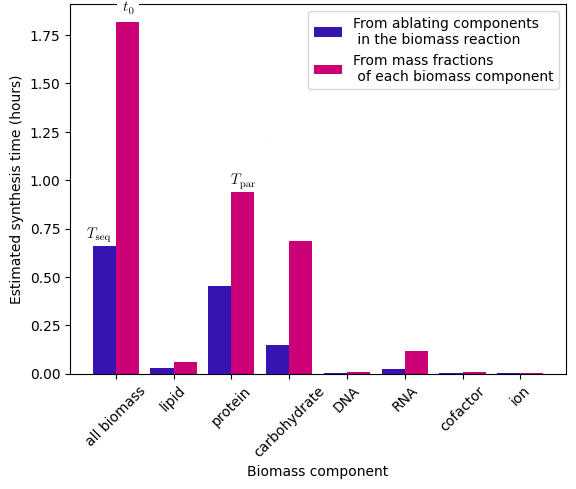
\includegraphics[width=.9\linewidth]{ablation_example_adapted.png}
  \caption{
    Comparing time scales derived from ablating components of the biomass reaction (blue) and from assuming that synthesis time is proportional to the mass fraction of the biomass component (red).
    % For each biomass component, the time $\Tiabl$ was computed according to equation~\ref{eq:model-ablated-time} (blue bars apart from leftmost column), and the time $\Tiprop$ was computed according to equation~\ref{eq:model-proportional-time} (red bars apart from leftmost column).
    % $\Tpar$ is defined as the greatest $\Tiprop$ (equation~\ref{eq:model-b}).
    % Blue under `all biomass' is $\Tseq$ (equation~\ref{eq:model-a}), the sum of times derived from ablation (other blue bars).
    % Red under `all biomass' is the doubling time $t_{0}$ (equation~\ref{eq:model-doubling-time}).
  }
  \label{fig:model-ablate-times}
\end{figure}


To evaluate whether sequential or parallel synthesis of biomass components offers a time advantage during cell growth, I estimated the timescale of biosynthesis for either resource allocation strategy (Fig.\ \ref{fig:model-ablate-times}).

Based on the objective function of the unmodified model, the doubling time is computed as follows:

\begin{equation}
  t_{0} = \frac{\ln 2}{\gro}
  \label{eq:model-doubling-time}
\end{equation}

where $t_{0}$ is the doubling time and $\gro$ is the growth rate, equivalent to the optimised flux of the biomass reaction.

Based on the growth rates computed in rounds of ablation (Fig.\ \ref{fig:model-ablate-fluxes}), the synthesis time of each biomass component is computed as follows:

\begin{equation}
  \Tiabl = f_{i} \cdot \frac{\ln 2}{\griabl}
  \label{eq:model-ablated-time}
\end{equation}

where:
\begin{itemize}
  \item $i$ represents each of the biomass components (lipids, proteins, carbohydrates, DNA, RNA, cofactors, and ions),
  \item $\Tiabl$ is the predicted time for synthesis of each biomass component,
  \item $f_{i}$ is the mass fraction of each biomass component, and
  \item $\griabl$ is the optimal flux of the ablated biomass reaction.
\end{itemize}

Eq.\ \ref{eq:model-ablated-time} differs from Eq.\ \ref{eq:model-doubling-time} in that $f_{i}$ acts as a scaling factor that takes into account that if a biomass component accounts for a smaller fraction of dry cell mass, biomass synthesis should take less time.
This value $f_{i}$ for each biomass component (table~\ref{tab:model-biomfrac}) is computed by dividing the molecular weight of the corresponding pseudometabolite by the molecular weight of biomass (table~\ref{tab:ecyeast8-mol-weights}).

\begin{table}[ht]
  \centering
  \begin{tabular}{lS}
    Metabolite & {$f_{i}$} \\
    \hline
    Protein & 0.52453 \\
    Carbohydrate & 0.36438 \\
    RNA & 0.06660 \\
    Lipid & 0.03283 \\
    Cofactors & 0.00502 \\
    DNA & 0.00406 \\
    Ions & 0.00258 \\
  \end{tabular}
  \caption{
    $f_{i}$ values for each biomass component.
  }
  \label{tab:model-biomfrac}
\end{table}


For comparison, I computed estimates of the time for each biomass component, assuming that it is proportional to the mass fraction:

\begin{equation}
  \Tiprop = f_{i} \cdot t_{0}
  \label{eq:model-proportional-time}
\end{equation}

where $t_{0}$ is the doubling time found in Eq.\ \ref{eq:model-doubling-time}.

To determine whether sequential biosynthesis of biomass components or parallel biosynthesis of biomass components is advantageous, I devise a ratio $\ratioabl$ that represents the ratio between the total time predicted by ablation and the biomass component that is predicted to take the most time.
This is defined:

\begin{equation}
  \ratioabl \coloneqq \frac{\Tseq}{\Tpar}
  \label{eq:model-ratio-simplified}
\end{equation}

where $\Tseq$ represents the predicted growth time assuming sequential biosynthesis and $\Tpar$ represents the limiting biomass synthesis time assuming parallel biosynthesis.
These quantities are defined:

\begin{equation}
  \Tseq \coloneqq \sum_{i} \Tiabl = \sum f_{i} \cdot \frac{\ln 2}{\griabl}
  \label{eq:model-a}
\end{equation}

% \begin{equation}
%   \begin{aligned}
%     \Tpar \coloneqq \argmax_{i} \Tiprop = \Tabl{protein} = \biomfrac{protein} \cdot \frac{\ln 2}{\gro},\\
%     \because \argmax_{i} f_{i} = \biomfrac{protein}
%   \end{aligned}
%   \label{eq:model-b}
% \end{equation}

\begin{equation}
  \Tpar \coloneqq \argmax_{i} \Tiprop
  \label{eq:model-b}
\end{equation}

As $\biomfrac{protein} = 0.525$, $\Tpar = \Tprop{protein}$.

Therefore,

\begin{equation}
  \begin{aligned}
    \ratioabl &= \frac{\Tseq}{\Tpar} \\
    & = \left( \sum_i \frac{f_i}{\griabl} \right) \cdot \frac{\gro}{\biomfrac{protein}} \\
    & = \left( \frac{\biomfrac{lipid}}{\grabl{lipid}} + \frac{\biomfrac{protein}}{\grabl{protein}} + \ldots + \frac{\biomfrac{ion}}{\grabl{ion}} \right) \cdot \frac{\gro}{\biomfrac{protein}}
    \end{aligned}
  \label{eq:model-ratio}
\end{equation}

The expression in Eq.\ \ref{eq:model-ratio} means that the definition of the $\ratioabl$ ratio does not reduce to a trivial expression and depends on the $\gro$ and the $\griabl$ values, which are all independent of each other.
%This relationship between $\ratioabl$ and $\gro$ and $\griabl$ is explored in section~\ref{sec:model-pool}.
A $\ratioabl < 1$ means that synthesising biomass components in sequence saves more time, favouring sequential biosynthesis.
Conversely, $\ratioabl > 1$ indicates that parallel synthesis of biomass components is favoured as synthesising biomass components in sequence does not save time.


\begin{figure}
  \centering
  \begin{subfigure}[htpb]{0.45\textwidth}
   \centering
   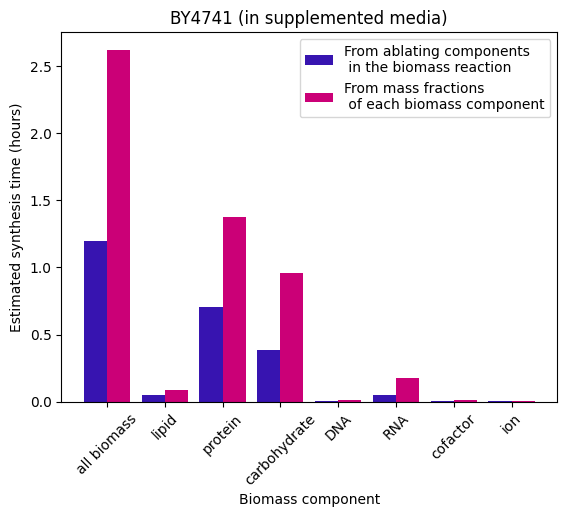
\includegraphics[width=\textwidth]{ablation_by4741}
   \caption{
     BY4741
   }
   \label{fig:model-ablation-by4741}
  \end{subfigure}
  \begin{subfigure}[htpb]{0.45\textwidth}
   \centering
   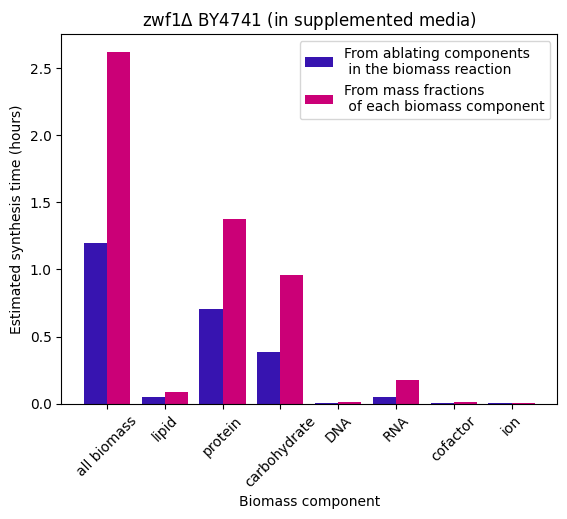
\includegraphics[width=\textwidth]{ablation_zwf1}
   \caption{
     zwf$\Delta$ in the BY4741 background.
   }
   \label{fig:model-ablation-zwf1}
  \end{subfigure}
  \begin{subfigure}[htpb]{0.45\textwidth}
   \centering
   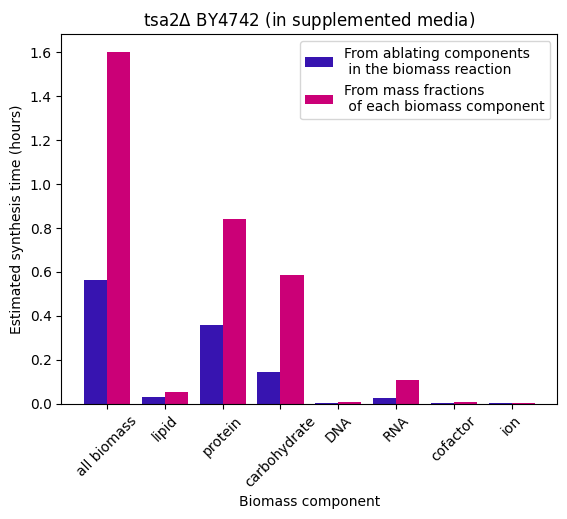
\includegraphics[width=\textwidth]{ablation_tsa2}
   \caption{
     tsa2$\Delta$ in the BY4742 background.  The ecYeast8 model does not include reactions that correspond to \textit{TSA1}.
   }
   \label{fig:model-ablation-tsa2}
  \end{subfigure}
  \caption{
    Comparing time scales from sequential and parallel biosynthesis in auxotrophs and deletion strains, as in figure~\ref{fig:model-ablate-times}.
    % For BY4741-background strains, supplements are simulated by allowing uptake of histidine, leucine, tryptophan, methionine and uracil.
    % The same applied to BY4742-background strains, but lysine uptake replaces methionine uptake.
  }
  \label{fig:model-ablation-strains}
\end{figure}
% Adding supplements, e.g. amino acids, dNTPs/NTPs, pyruvate, glucose limitation?
% Or do C/N grid heatmaps demonstrate this.

% In figure~\ref{fig:model-ablate-times}, the $\ratioabl = 0.70$.
To confirm that the advantage of the sequential biosynthesis strategy is retained in other strains, I extended the computation $\ratioabl$ and related quantities to models in which genes were deleted.
In accordance with chapter 3, the BY4741 zwf1$\Delta$ and BY4742 tsa1$\Delta$ tsa2$\Delta$ strains were simulated.
The deletions were made by restricting reaction fluxes that are associated with the deleted genes to zero.
For BY4741-background strains, supplements are simulated by allowing uptake of histidine, leucine, tryptophan, methionine and uracil.
The same applied to BY4742-background strains, but lysine uptake replaces methionine uptake.
Fig.\ \ref{fig:model-ablation-strains} shows that $\ratioabl < 1$ still holds for auxotrophs and deletion strains, suggesting that the sequential biosynthesis strategy remains advantageous.
Assuming that temporal scheduling of the synthesis of biomass components during growth explains the timing of biosynthetic events in the yeast metabolic cycle, these observations supports results in chapter 3 which shows that auxotrophs and deletion strains have YMCs.


\section{Effect of restricting the enzyme pool}
\label{sec:model-pool}

The yeast cell has a finite enzyme-available proteome pool, so it must decide which enzymes to allocate the greatest proportions of the pool to, for enzyme synthesis.
In order to study this effect using the ecYeast8 model, a constraint on the proteome pool must be imposed, and I imposed this constraint by varying the enzyme-available proteome pool defined by the enzyme pool pseudoreaction (Eq.\ \ref{eq:model-gecko-enzyme-pool-flux}).
To vary the enzyme-available proteome pool in the ecYeast8 model,
I vary the value of the upper limit of the flux $\epool$ of the enzyme pool pseudoreaction (equation~\ref{eq:model-gecko-enzyme-pool}) in order to change the flux available for enzyme usage pseudoreactions (equation~\ref{eq:model-gecko-enzyme-usage}).
With a smaller $\epool$, the sum of fluxes of enzyme usage pseudoreactions must decrease, and the model must decide which enzyme usage pseudoreactions to allocate a higher flux to, modelling the biological response to a restricted enzyme pool.

% TODO: Clarify what sort of changes need to be made, especially in the text.  I struggle to understand what the better alternative should be like, at the moment.
\begin{figure}
  \centering
  \begin{subfigure}[htpb]{0.45\textwidth}
   \centering
   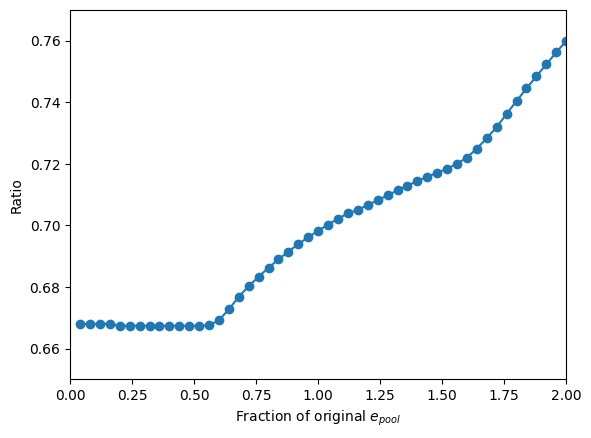
\includegraphics[width=\textwidth]{epool_ec_ratio_shrinkyaxis}
   \caption{
     Effect on ratio ($\ratioabl$), $\epool^{\prime}/\epool \leq 2$.
   }
   \label{fig:model-pool-ratio}
  \end{subfigure}%
  \begin{subfigure}[htpb]{0.45\textwidth}
   \centering
   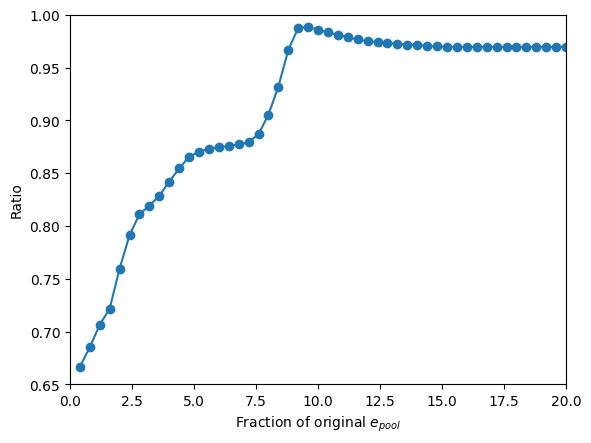
\includegraphics[width=\textwidth]{epool_ec_ratio_20_shrinkyaxis}
   \caption{
     Effect on ratio ($\ratioabl$), $\epool^{\prime}/\epool \leq 20$.
   }
   \label{fig:model-pool-ratio-20}
  \end{subfigure}

  \begin{subfigure}[htpb]{0.45\textwidth}
   \centering
   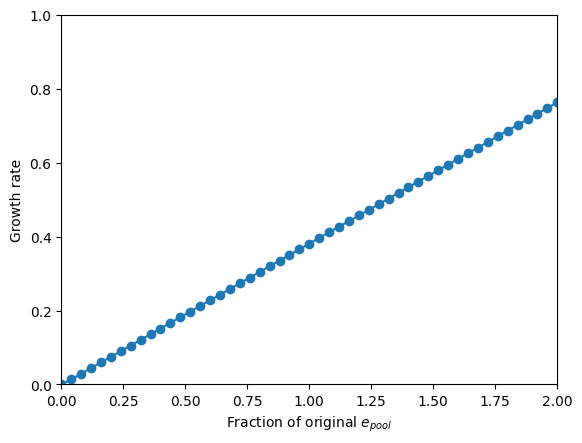
\includegraphics[width=\textwidth]{epool_ec_gr}
   \caption{
     Effect on wild type growth rate ($\gro$), $\epool^{\prime}/\epool \leq 2$.
   }
   \label{fig:model-pool-growthrate}
  \end{subfigure}%
  \begin{subfigure}[htpb]{0.45\textwidth}
   \centering
   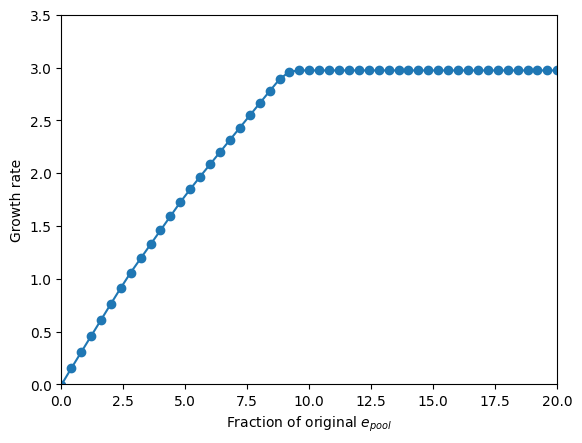
\includegraphics[width=\textwidth]{epool_ec_gr_20}
   \caption{
     Effect on wild type growth rate ($\gro$), $\epool^{\prime}/\epool \leq 20$.
   }
   \label{fig:model-pool-growthrate-20}
  \end{subfigure}

  \begin{subfigure}[htpb]{0.45\textwidth}
   \centering
   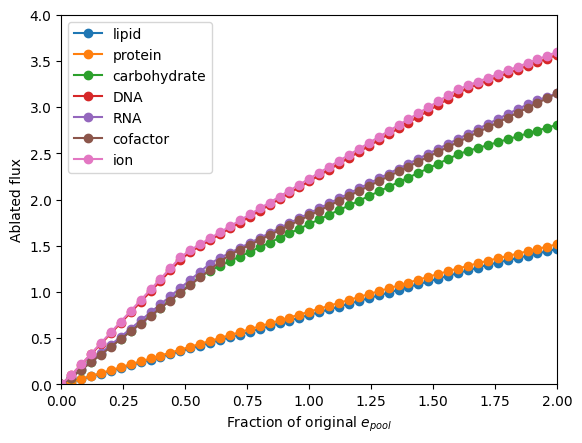
\includegraphics[width=\textwidth]{epool_ec_components}
   \caption{
     Effect on ablated growth rates ($\griabl$), $\epool^{\prime}/\epool \leq 2$.
   }
   \label{fig:model-pool-ablated}
  \end{subfigure}%
  \begin{subfigure}[htpb]{0.45\textwidth}
   \centering
   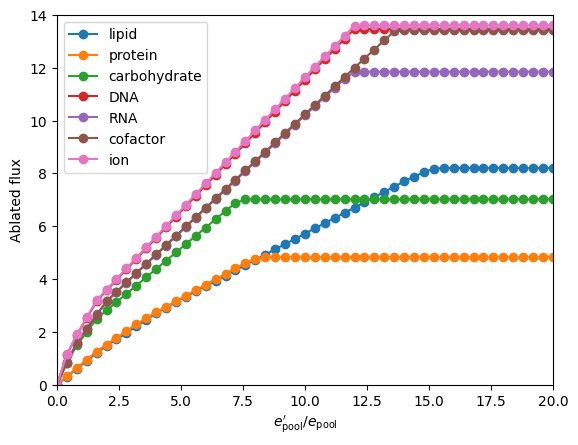
\includegraphics[width=\textwidth]{epool_ec_components_20}
   \caption{
     Effect on ablated growth rates ($\griabl$), $\epool^{\prime}/\epool \leq 20$
   }
   \label{fig:model-pool-ablated-20}
  \end{subfigure}

  \caption{
    Effect of the size of the proteome pool available for enzymes ($\epool^{\prime}$) on $\ratioabl$ and growth rates.
    % Constraining the proteome pool available for synthesis enzymes leads to a greater advantage of sequential biosynthesis of biomass components over parallel biosynthesis, as evidenced by a decreasing $\ratioabl$ ratio if $\epool^{\prime}$ decreases (\ref{fig:model-pool-ratio}).
    % Concurrently, as $\epool^{\prime}$ decreases, the wild type growth rate ($\gro$) decreases linearly to zero (\ref{fig:model-pool-growthrate}) and ablated growth rates ($\griabl$) decrease in linear segments independently of each other and of the growth rate (\ref{fig:model-pool-growthrate}).
    % These values determine the ratio according to equation~\ref{eq:model-ratio}.
  }
  \label{fig:model-pool}
\end{figure}

Fig.\ \ref{fig:model-pool} shows that constraining the proteome pool available for enzymes leads to a greater advantage of sequential biosynthesis of biomass components over parallel biosynthesis, as evidenced by a decreasing $\ratioabl$ ratio if $\epool^{\prime}$ decreases.
Concurrently, as $\epool^{\prime}$ decreases, the wild type growth rate ($\gro$) decreases linearly to zero (Fig.\ \ref{fig:model-pool-growthrate}) and ablated growth rates ($\griabl$) decrease in linear segments independently of each other and of the growth rate (Fig.\ \ref{fig:model-pool-growthrate}).
These observations can be explained by considering Eq.\ \ref{eq:model-ratio} and modelling changes in $\gro$ and $\griabl$ with respect to $\epool^{\prime}/\epool$ as linear equations (Appendix \ref{append:model-pool}).

% FIXME: Make this less like a lecture and link interpretations to hypotheses/etc.
Figure~\ref{fig:model-pool} shows the results of my investigation.
% In full: 0.103697326777848
I denote $\epool$ as the default enzyme-available proteome pool (\SI{0.104}{\gram~\gram_{DW}^{-1}}) and $\epool^{\prime}$ as the enzyme-available proteome pool I set in the model.
When $0 \leq \epool^{\prime} \leq 2\epool$, the model gives realistic growth rates \SIrange{0}{0.8}{\hour^{-1}} (figure~\ref{fig:model-pool-growthrate}).
In this region, growth rate increases linearly as $\epool$ increases.
With higher $\epool^{\prime}$ values --- that is, less of a constraint on the enzyme pool --- the $\ratioabl$ ratio increases, thus indicating that sequential biosynthesis gives less of an advantage (figure~\ref{fig:model-pool-ratio}).
As $\epool^{\prime}$ increases, ablated growth rates $\griabl$ increases linearly at low $\epool^{\prime}$ (figure~\ref{fig:model-pool-ablated}).
But then, at higher $\epool^{\prime}$, these linear relationships decrease in gradient, all going to a plateau at very high $\epool^{\prime}$ (figure~\ref{fig:model-pool-ablated-20}).
This behaviour shows that the relationship between $\griabl$ and $\epool^{\prime}$ is independent of the growth rate $\gro$ and of each other.
% TODO: Come up with a better (biological) interpretation -- consult some org notes.
The $\griabl$ of different components plateau at different $\epool^{\prime}$ sizes, with carbohydrate reaching a plateau first, followed by protein.
This may indicate that the enzyme-available proteome pool is limiting for these components, which may be because the cell needs more enzyme mass to catalyse the reactions needed for the synthesis of these components.


\section{Effect of carbon and nitrogen sources}
\label{sec:model-exchange}

% FIXME: Be consistent in referring to exchange rate/saturation.  Come up with some phrase to use.
\subsection{Saturation of exchange reactions}
\label{subsec:model-saturation}

To explore whether sequential synthesis of biomass components remains advantageous across nutrient conditions, in addition to across gene deletion strains, I investigate how changes in the concentrations of carbon and nitrogen sources affect the resource allocation strategy in yeast.
I investigated ammonium as a nitrogen source as it is the form of nitrogen in minimal growth media, and investigates two carbon sources: glucose and pyruvate.
Glucose is the preferred carbon source for budding yeast, while studying pyruvate would give an insight into a non-fermentable carbon source.

In order to conduct this investigation using FBA, ranges of nutrient exchange fluxes that are suitable for the model need to be found.
Genome-scale metabolic models include nutrient exchange reactions whose flux bounds can be unrestricted to simulate the presence of certain nutrients in the growth medium.
% FIXME: This sentence
In contrast to simulating the presence or absence of nutrients, simulating a certain concentration of a nutrient requires setting specific flux bounds.
Because FBA does not account for substrate concentrations, the concentration of nutrients cannot directly be used to set flux bounds.
Instead, studies constrain the flux of exchange reactions in such a way that the optimised growth rate matches experimental observations \parencite{elsemmanWholecellModelingYeast2022}.
% TODO: Find other studies that did the same and cite them here.


\begin{figure}
  \centering
  \begin{subfigure}[t]{0.45\textwidth}
  \centering
    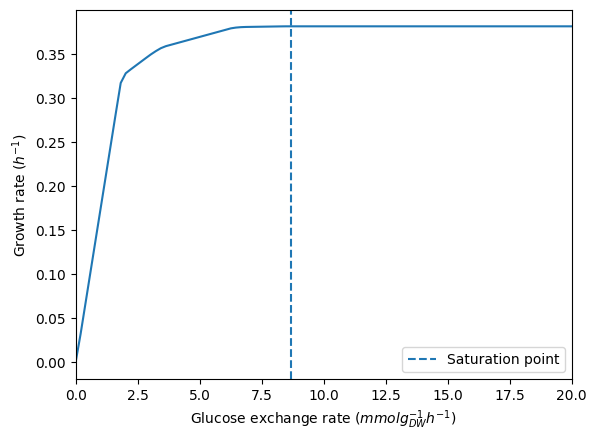
\includegraphics[width=\linewidth]{saturation_glc}
    \caption{
      % Effect of glucose exchange on growth rate, with ammonium exchange flux unrestricted.
      % Growth rate saturation is at \SI{8.69}{\mmolgdwh}.
    }
    \label{fig:model-saturation-glucose}
  \end{subfigure}%
  \begin{subfigure}[t]{0.45\textwidth}
  \centering
    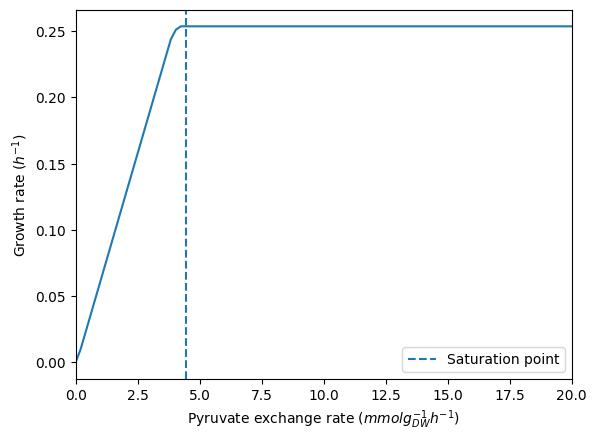
\includegraphics[width=\linewidth]{saturation_pyr}
    \caption{
      % Effect of pyruvate exchange on growth rate, with ammonium exchange flux unrestricted.
      % Growth rate saturation is at \SI{4.44}{\mmolgdwh}.
    }
    \label{fig:model-saturation-pyruvate}
  \end{subfigure}

  \begin{subfigure}[t]{0.45\textwidth}
  \centering
    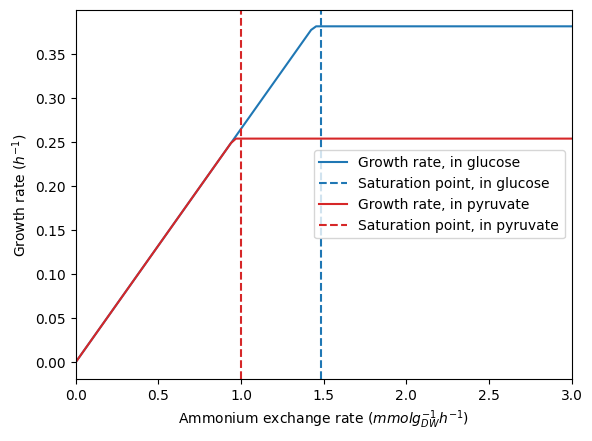
\includegraphics[width=\linewidth]{saturation_amm}
    \caption{
      % Effect of ammonium exchange on growth rate, with exchanges of carbon sources set to growth rate saturation based on figures~\ref{fig:model-saturation-glucose} and ~\ref{fig:model-saturation-pyruvate}.
      % Growth rate saturation is at \SI{1.48}{\mmolgdwh} in glucose, and
      % at \SI{1.00}{\mmolgdwh} in pyruvate.
    }
    \label{fig:model-saturation-ammonium}
  \end{subfigure}

  \caption{
    Effect of glucose (\ref{fig:model-saturation-glucose}), pyruvate (\ref{fig:model-saturation-pyruvate}), and ammonium (\ref{fig:model-saturation-ammonium}) exchange reactions on growth rate.
  }
  \label{fig:model-saturation}
\end{figure}

The saturation point of exchange reactions functions as a useful reference for exchange reaction flux values.
This saturation point is defined as the flux of an exchange reaction above which the objective function reaches its maximum.
Fig.\ \ref{fig:model-saturation} shows growth saturation curves that illustrate the effect of glucose, pyruvate, and ammonium exchange rates on the growth rate.
Simulation results show that the maximum growth rate on glucose (\SI{0.38}{\hour^{-1}}) is greater than the maximum growth rate on pyruvate (\SI{0.25}{\hour^{-1}}), and
the growth rate saturation point for ammonium is determined by the maximal growth rate on the carbon source (Fig.\ \ref{fig:model-saturation-ammonium}).

These growth saturation curves agree with similar studies.
Specifically, the growth saturation curve for glucose (Fig.\ \ref{fig:model-saturation-glucose}) is similar to that simulated by \textcite{elsemmanWholecellModelingYeast2022} using another derivative of the Yeast8 model.
The maximum growth rate on glucose agrees with \textcite{domenzainReconstructionCatalogueGenomescale2022}, which used GECKO 2 to create the ecYeast7 model to predict maximum growth rates on various carbon sources.
\textcite{domenzainReconstructionCatalogueGenomescale2022} did not simulate growth on pyruvate, but a lower maximum growth rate on pyruvate is consistent with my experimental observations.


\subsection{Effect of carbon and nitrogen sources on biomass synthesis strategies}
\label{subsec:model-grid}

\subsubsection{Glucose and ammonium}
\label{subsec:model-grid-glucose}

\begin{figure}
  \centering
  \begin{subfigure}[t]{0.45\textwidth}
  \centering
    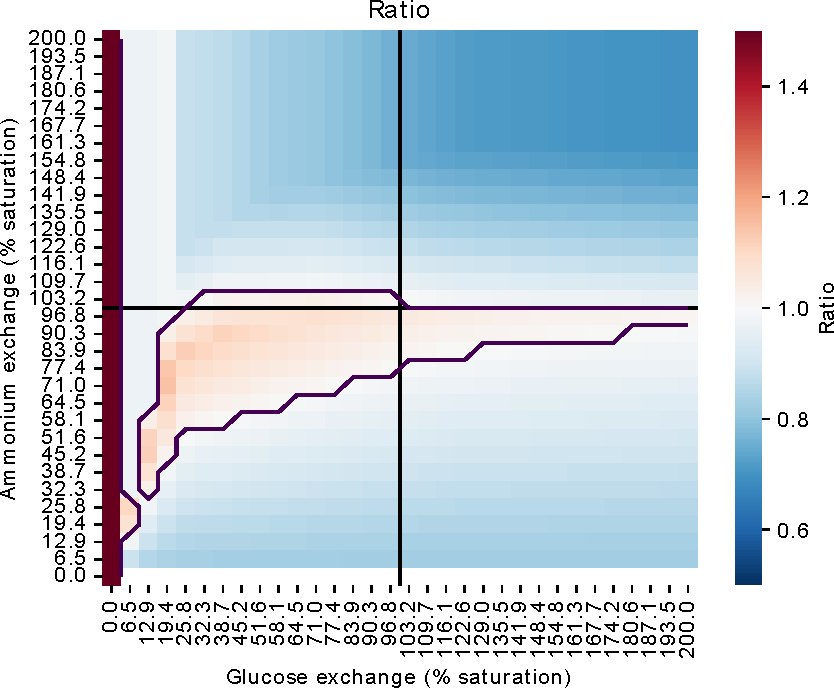
\includegraphics[width=\linewidth]{ec_grid_glc_amm_ratio}
    \caption{
      Ratio ($\ratioabl$)
    }
    \label{fig:model-grid-glc-ratio}
  \end{subfigure}%
  \begin{subfigure}[t]{0.45\textwidth}
  \centering
    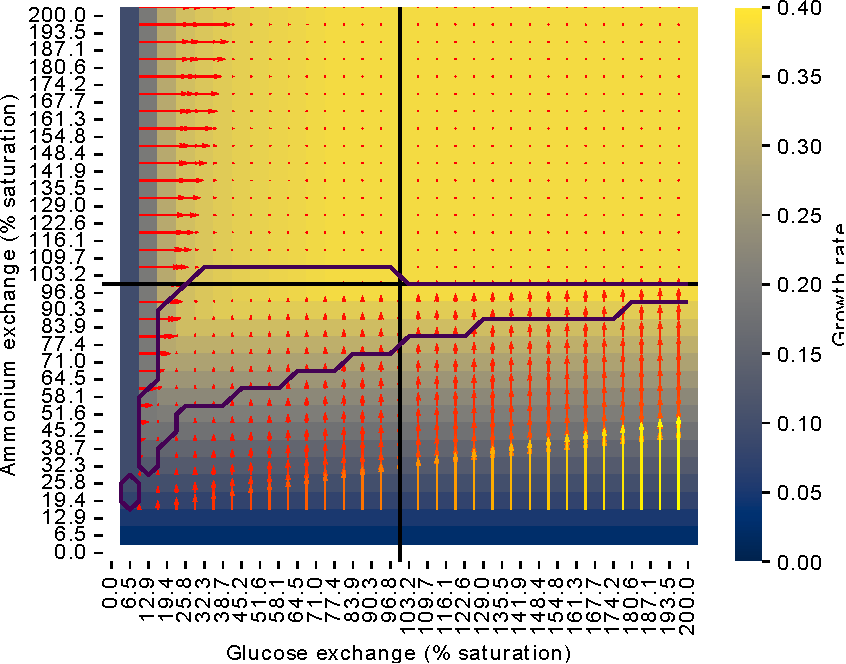
\includegraphics[width=\linewidth]{ec_grid_glc_amm_gr}
    \caption{
      Growth rate based on unmodified biomass reaction ($\gro$)
    }
    \label{fig:model-grid-glc-growthrate}
  \end{subfigure}

  \begin{subfigure}[t]{0.45\textwidth}
  \centering
    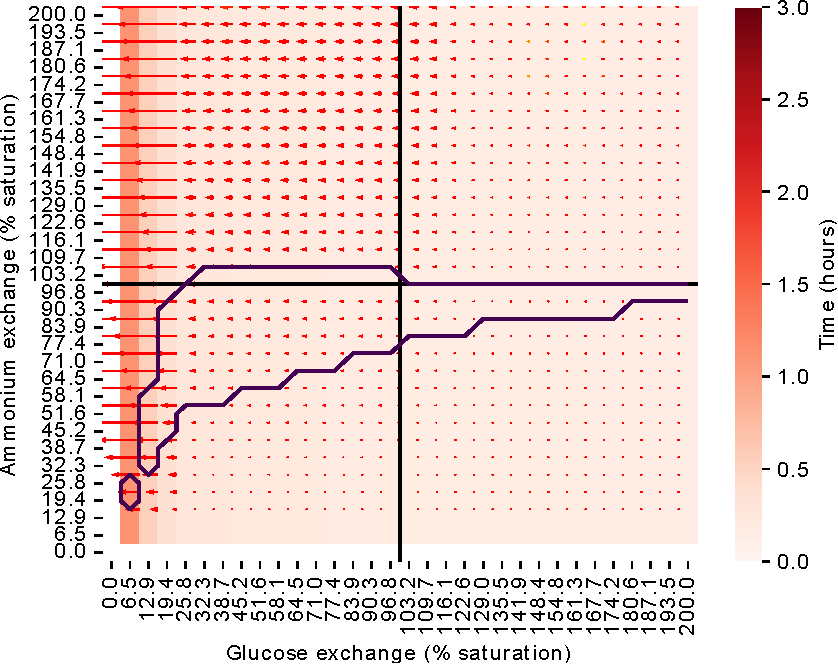
\includegraphics[width=\linewidth]{ec_grid_glc_amm_carb}
    \caption{
      Predicted carbohydrate synthesis time ($\Tabl{carbohydrate}$)
    }
    \label{fig:model-grid-glc-carb}
  \end{subfigure}%
  \begin{subfigure}[t]{0.45\textwidth}
  \centering
    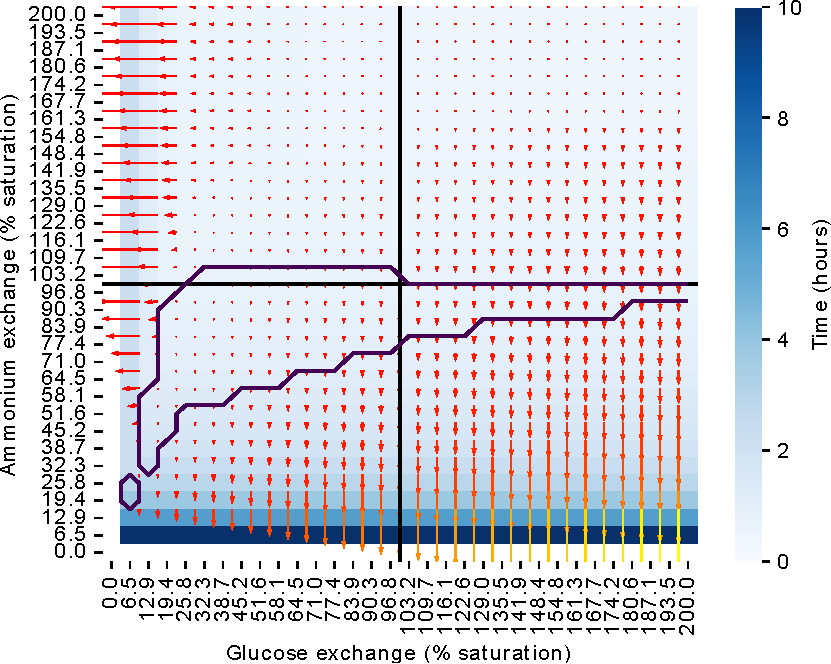
\includegraphics[width=\linewidth]{ec_grid_glc_amm_prot}
    \caption{
      Predicted protein synthesis time ($\Tabl{protein}$)
    }
    \label{fig:model-grid-glc-prot}
  \end{subfigure}

  \begin{subfigure}[t]{0.45\textwidth}
  \centering
    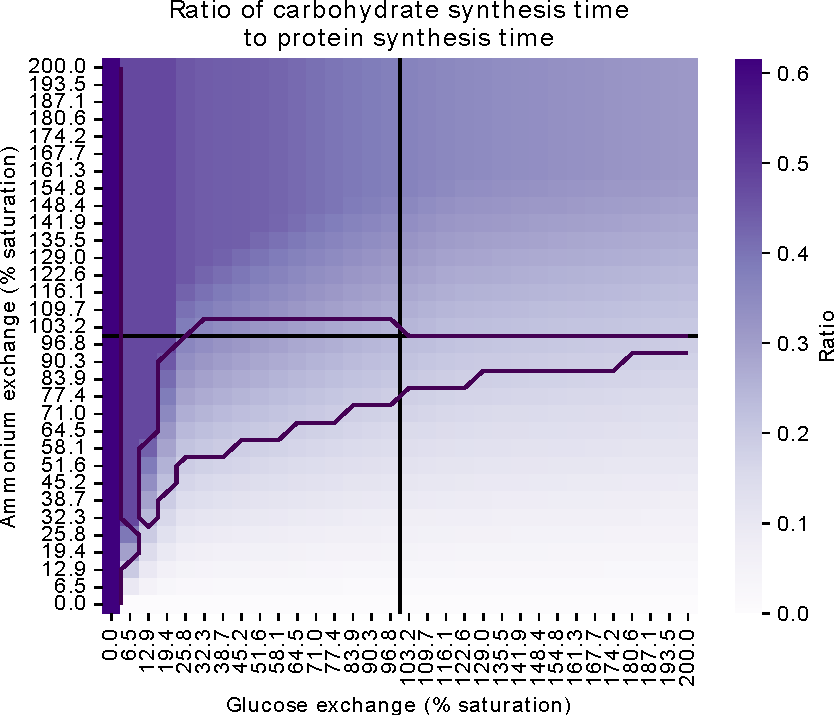
\includegraphics[width=\linewidth]{ec_grid_glc_amm_carb_to_prot}
    \caption{
      Ratio of carbohydrate synthesis time to protein synthesis time ($\Tabl{carbohydrate}/\Tabl{protein}$)
    }
    \label{fig:model-grid-glc-carb-to-prot}
  \end{subfigure}
  \caption{
    Effect of glucose ($\exchrate{glc}$) and ammonium exchange rates ($\exchrate{amm}$) on various quantities.
    Exchange rates are expressed in percentages of growth saturation from in Fig.\ \ref{fig:model-saturation}, with black straight lines indicate 100\% of saturation.
    Contours show regions in which $\ratioabl > 1$.
    Arrows indicate susceptibility of the quantity displayed in the heatmap, relative to $\exchrate{glc}$ and $\exchrate{amm}$.
  }
  \label{fig:model-grid-glc}
\end{figure}

To assess the effect of glucose and ammonium concentration on biomass synthesis strategies, I ablated components in the biomass reaction in different nutrient conditions set by glucose and ammonium exchange
to obtain $\ratioabl$, $\gro$, $\Tabl{carbohydrate}$, and $\Tabl{protein}$ (Fig.\ \ref{fig:model-grid-glc}).
Whether $\ratioabl$ was less than or greater than 1 indicated whether the sequential or parallel strategy is advantageous for each condition. %, while $\gro$ indicated which nutrient source was limiting in each condition.
Synthesis times $\Tiabl$ were computed to assess whether the ratio between the synthesis times differed in different conditions, in particular, conditions in which parallel biomass synthesis is favoured ($\ratioabl > 1$).
The ratio $\frac{\Tabl{carbohydrate}}{\Tabl{protein}}$ serves as the principal measure to quantify how $\Tiabl$ values change as carbon and nitrogen source concentrations change.
This ratio between $\Tabl{carbohydrate}$ and $\Tabl{protein}$ is informative because:
\begin{enumerate}
  \item Of all biomass components, predicted synthesis times of these biomass components varied the most as the glucose and ammonium exchange rates were varied.
  \item Each accounts for a large proportion of biomass: protein accounts for 52.5\% and carbohydrate accounts for 36.4\% (table~\ref{tab:ecyeast8-mol-weights}).
  \item Carbohydrate synthesis has a clear biochemical relationship with the level of a carbon source.
        And, because amino acids contain amino groups, protein synthesis has a biochemical relationship with ammonium as a nitrogen source.
\end{enumerate}

To determine whether the carbon or nitrogen source is limiting for each of the quantities calculated, I defined the sensitivity at each nutrient condition $(\exchrate{glc}, \exchrate{amm})$, with respect to each axis $i$ as:

\begin{equation}
  s_{i}(\exchrate{glc}, \exchrate{amm}) = \frac{R_{i}}{y(\exchrate{glc}, \exchrate{amm})} \cdot \pdif{y(\exchrate{glc}, \exchrate{amm})}{R_{i}}
  \label{eq:model-susceptibility}
\end{equation}

where:
\begin{itemize}
  \item $i$ indicates glucose (glc) or ammonium (amm)
  \item $R_{i}$ indicates the exchange rate, glucose ($\exchrate{glc}$) or ammonium ($\exchrate{amm}$).
        An $(\exchrate{glc}, \exchrate{amm})$ pair defines a nutrient condition.
  \item $y(\exchrate{glc}, \exchrate{amm})$ represents the quantity of interest at each nutrient condition
\end{itemize}

At a specific nutrient condition $(\exchrate{glc}, \exchrate{amm})$, if $s_{\mathrm{glc}}(\exchrate{glc}, \exchrate{amm}) > s_{\mathrm{amm}}(\exchrate{glc}, \exchrate{amm})$ for a quantity of interest $y$, then it means that the quantity is more sensitive to --- or more limited by --- glucose exchange at this condition.
The reverse is true if $s_{\mathrm{glc}}(\exchrate{glc}, \exchrate{amm}) < s_{\mathrm{amm}}(\exchrate{glc}, \exchrate{amm})$.
To visualise the extent to which each exchange rate limits each quantity of interest, I show the sensitivity values as arrows (Figs.\ \ref{fig:model-grid-glc} and~\ref{fig:model-grid-pyr}) with $s_{\mathrm{glc}}$ and $s_{\mathrm{amm}}$ as two components of the vector that defines these arrows.
Thus, horizontal arrows indicate a strong sensitivity to glucose and vertical arrows indicate a strong sensitivity to ammonium, while the arrows point towards increasing values of the quantity of interest.

Figs.\ \ref{fig:model-grid-glc-ratio} and~\ref{fig:model-grid-glc-growthrate} show that the region where $\ratioabl > 1$ corresponds to a region around the boundary between the region where glucose more limits growth rate and the region where ammonium more limits growth rate, plus a region where ammonium exchange is a saturation while glucose exchange is over saturation.
In contrast, when the growth rate is near its maximum, where neither glucose nor ammonium is limiting, when glucose or ammonium exchange increases, sequential biosynthesis becomes more advantageous.

To explain why $\ratioabl > 1$ when ammonium exchange is under saturation and glucose is over saturation, consider equation~\ref{eq:model-ratio}.
If we assume that $\frac{f_i}{\griabl}$ for $i$ other than carbohydrate and protein changes negligibly --- justified by the small $f_{i}$ values for these other biomass components --- we write:

\begin{equation}
  \ratioabl \approx (k + \frac{\biomfrac{protein}}{\grabl{protein}} + \frac{\biomfrac{carbohydrate}}{\grabl{carbohydrate}}) \cdot \frac{\gro}{\biomfrac{protein}}
  \label{eq:model-ratio-assume}
\end{equation}

where $k$ is a constant.

In the glucose-limiting region, as $\exchrate{glc}$ increases, under saturation,
\begin{itemize}
  \item $\gro$ increases,
  \item $\grabl{carbohydrate}$ increases, and
  \item $\grabl{protein}$ increases, while
  \item $\ratioabl$ stays constant.
\end{itemize}

In the nitrogen-limiting region, as $\exchrate{amm}$ increases, under saturation,
\begin{itemize}
  \item $\gro$ increases,
  \item $\grabl{carbohydrate}$ stays constant, and
  \item $\grabl{protein}$ increases, while
  \item $\ratioabl$ increases.
\end{itemize}

Based on the glucose-limiting region, the increases in $\grabl{carbohydrate}$ and $\grabl{protein}$ in the carbon-limiting case are just enough to balance the increase in $\gro$.
Then, in the nitrogen-limiting case, if there is no increase in $\grabl{carbohydrate}$, then the combined effect of $\grabl{carbohydrate}$ and $\grabl{protein}$ no longer balance the increase in $\gro$.
This thus explains why $\ratioabl$ increases in this case.

If both nutrients are limiting, as $(\exchrate{glc}, \exchrate{amm})$ varies along the curve from $(0, 0)$ to $(\exchrate{glc, saturation}, \exchrate{amm, saturation})$ that goes through such conditions, both $\grabl{carbohydrate}$ and $\grabl{protein}$ increase, explaining why $\ratioabl$ remain roughly at the same high values greater than 1.
Thus, the region where $\ratioabl > 1$ where both glucose and ammonium are near-limiting can be seen as where the behaviour of the glucose-limiting and ammonium-limiting cases meet.

Next, I investigate $\frac{\Tabl{carbohydrate}}{\Tabl{protein}}$.

Based on equation~\ref{eq:model-ablated-time},

\begin{equation}
  \frac{\Tabl{carbohydrate}}{\Tabl{protein}} = \frac{\biomfrac{carbohydrate}}{\biomfrac{protein}} \cdot \frac{\grabl{protein}}{\grabl{carbohydrate}}
  \label{eq:model-carb-prot-ratio}
\end{equation}

In the glucose-limiting region, $\frac{\Tabl{carbohydrate}}{\Tabl{protein}}$ remains at a high value because, as $\exchrate{glc}$ increases in this region, both $\grabl{carbohydrate}$ and $\grabl{protein}$ increase.
However, in the ammonium-limited region, $\frac{\Tabl{carbohydrate}}{\Tabl{protein}}$ increases as $\exchrate{amm}$ increases because then $\grabl{protein}$ increases while $\grabl{carbohydrate}$ remains constant.
If both nutrients are limiting, as $(\exchrate{glc}, \exchrate{amm})$ varies along the curve from $(0, 0)$ to $(\exchrate{glc, saturation}, \exchrate{amm, saturation})$ that goes through such conditions, both $\grabl{carbohydrate}$ and $\grabl{protein}$ increase, explaining why $\frac{\Tabl{carbohydrate}}{\Tabl{protein}}$ remain roughly at the same.

Considering $\Tabl{carbohydrate}$ and $\Tabl{protein}$, glucose exchange limits carbohydrate synthesis time for virtually every nutrient condition.
In contrast, ammonium exchange limits protein synthesis time for most nutrient conditions, except for conditions in which glucose exchange is very low, owing to the fact that both carbon and nitrogen sources contribute to protein biosynthesis.
Taken together with the discussion above, these effects of nutrient exchange on protein and carbohydrate synthesis times thus explain the patterns of $\ratioabl$ and $\frac{\Tabl{carbohydrate}}{\Tabl{protein}}$ as both exchange reactions change in flux.

\subsubsection{Pyruvate and ammonium}
\label{subsec:model-grid-pyruvate}

\begin{figure}
  \centering
  \begin{subfigure}[t]{0.45\textwidth}
  \centering
    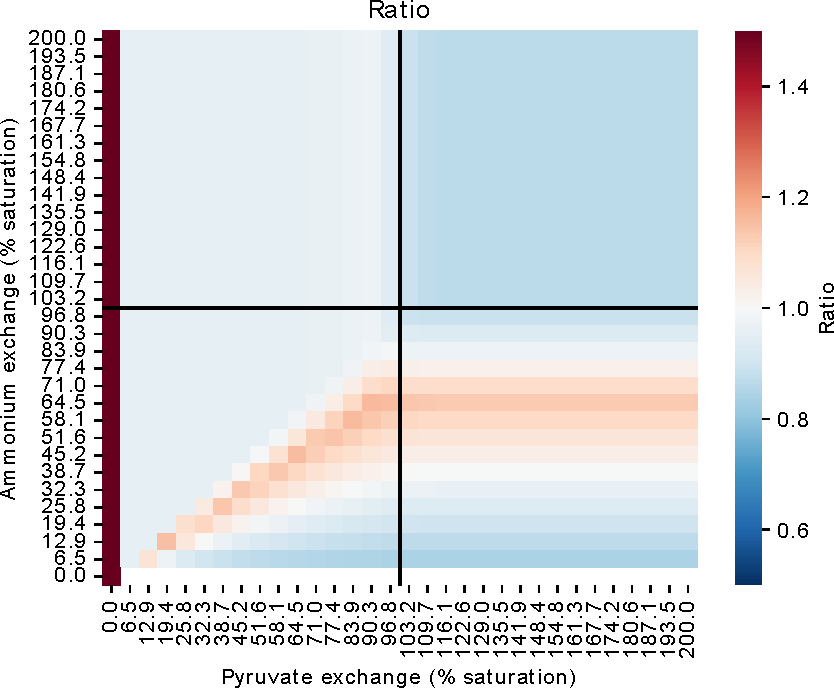
\includegraphics[width=\linewidth]{ec_grid_pyr_amm_ratio}
    \caption{
      Ratio ($\ratioabl$)
    }
    \label{fig:model-grid-pyr-ratio}
  \end{subfigure}%
  \begin{subfigure}[t]{0.45\textwidth}
  \centering
    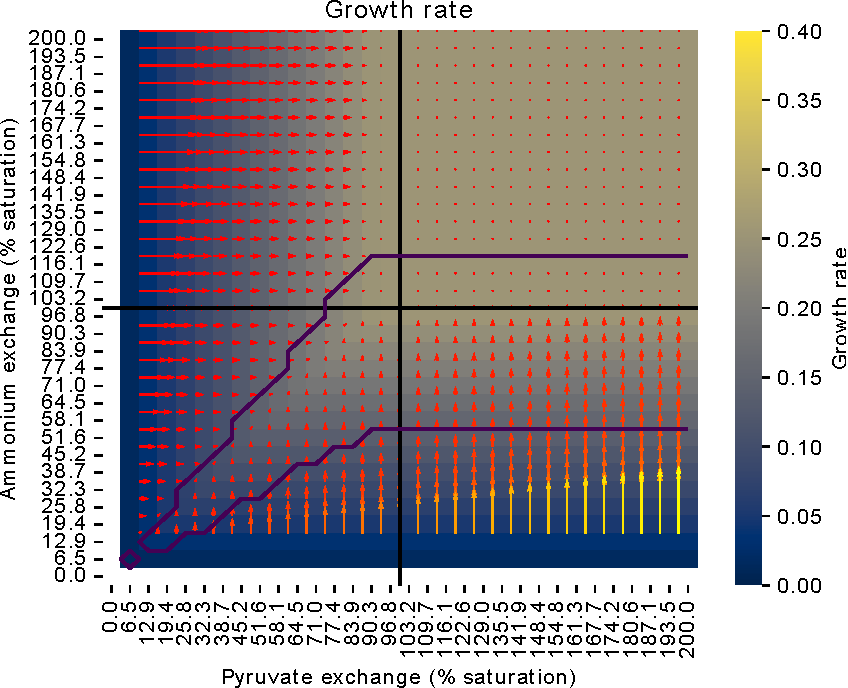
\includegraphics[width=\linewidth]{ec_grid_pyr_amm_gr}
    \caption{
      Growth rate based on unmodified biomass reaction ($\gro$)
    }
    \label{fig:model-grid-pyr-growthrate}
  \end{subfigure}

  \begin{subfigure}[t]{0.45\textwidth}
  \centering
    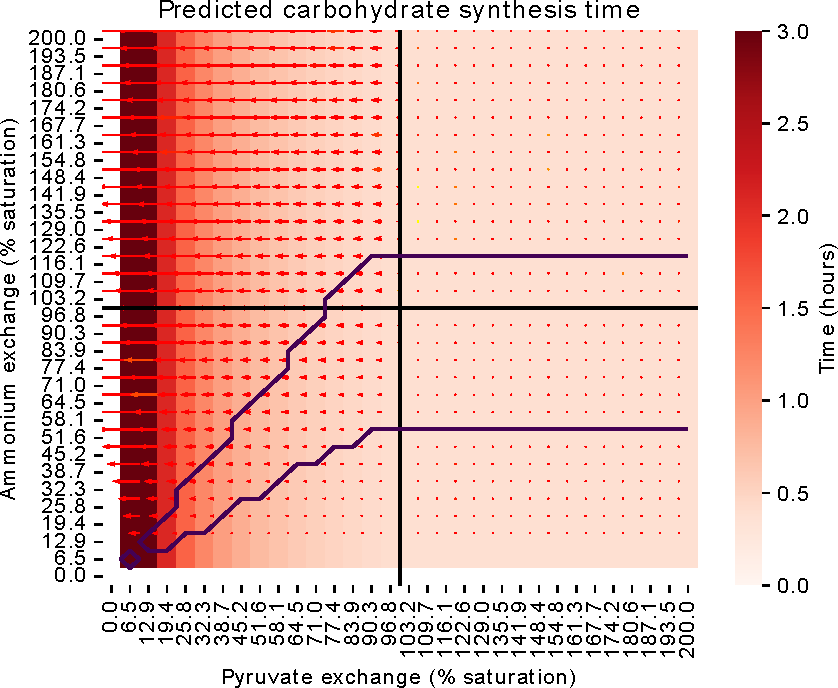
\includegraphics[width=\linewidth]{ec_grid_pyr_amm_carb}
    \caption{
      Predicted carbohydrate synthesis time ($\Tabl{carbohydrate}$)
    }
    \label{fig:model-grid-pyr-carb}
  \end{subfigure}%
  \begin{subfigure}[t]{0.45\textwidth}
  \centering
    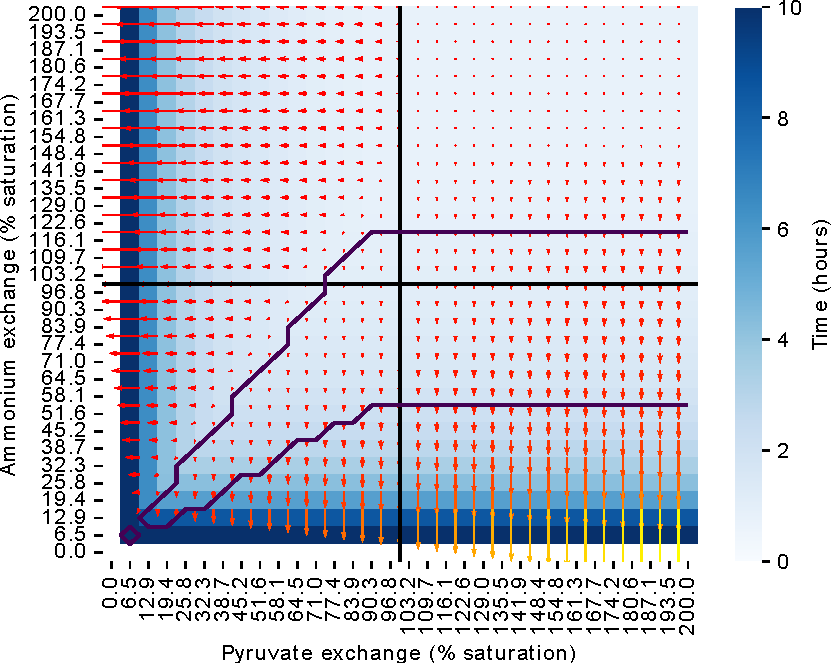
\includegraphics[width=\linewidth]{ec_grid_pyr_amm_prot}
    \caption{
      Predicted protein synthesis time ($\Tabl{protein}$)
    }
    \label{fig:model-grid-pyr-prot}
  \end{subfigure}

  \begin{subfigure}[t]{0.45\textwidth}
  \centering
    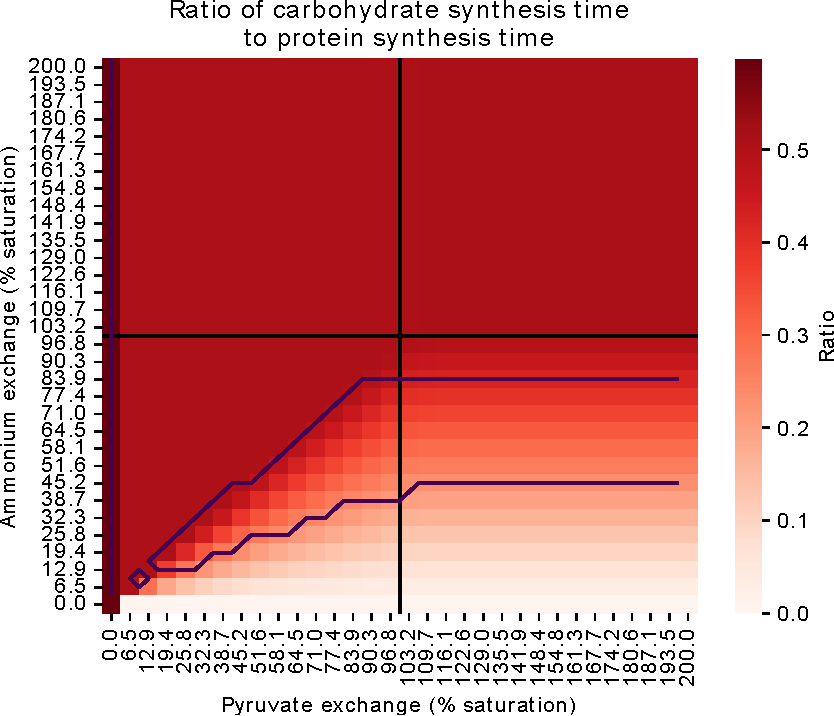
\includegraphics[width=\linewidth]{ec_grid_pyr_amm_carb_to_prot}
    \caption{
      Ratio of carbohydrate synthesis time to protein synthesis time ($\Tabl{carbohydrate}/\Tabl{protein}$)
    }
    \label{fig:model-grid-pyr-carb-to-prot}
  \end{subfigure}
  \caption{
    Effect of glucose ($\exchrate{pyr}$) and ammonium exchange rates ($\exchrate{amm}$) on various quantities.
    Exchange rates are expressed in percentages of growth saturation from in Fig.\ \ref{fig:model-saturation}, with black straight lines indicate 100\% of saturation.
    Contours show regions in which $\ratioabl > 1$.
    Arrows indicate susceptibility of the quantity displayed in the heatmap, relative to $\exchrate{pyr}$ and $\exchrate{amm}$.
  }
  \label{fig:model-grid-pyr}
\end{figure}

To investigate the effect on a non-fermentable carbon source, I repeated the investigation using pyruvate as the carbon source, and adjusted the saturation exchange rates accordingly: pyruvate saturation being at \SI{4.44}{\mmolgdwh} and ammonium saturation being at \SI{1.00}{\mmolgdwh} (figure~\ref{fig:model-grid-pyr}).
Overall, pyruvate seems to represent an extreme case of the glucose investigation.
The previous discussion of how the quantities of interest vary as exchange rates vary applies.
Though, the change of behaviour can be explained by how the growth saturation curve under pyruvate has a different shape from the growth saturation curve under glucose.


\subsection{Relationship between proteome allocation and resource allocation strategy}
\label{subsec:model-rank}

\subsubsection{Glucose and ammonium}
\label{subsec:model-rank-glucose}

\begin{figure}
  \centering
  \begin{subfigure}[t]{0.45\textwidth}
  \centering
    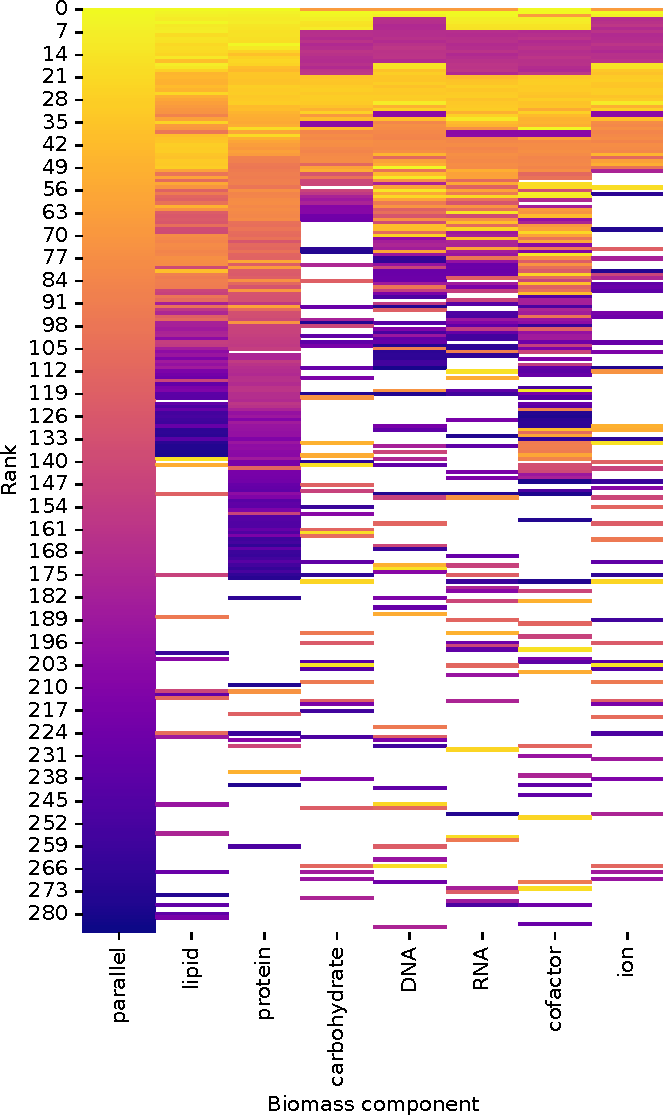
\includegraphics[width=\linewidth]{CompareEnzUse_glc16p89_pyrUnres_ammUnres_1.pdf}
    \caption{
      Rank of enzyme usage reactions in the low $\ratioabl$ case ($\exchrate{glucose}$ = \SI{16.89}{\mmolgdwh}).
    }
    \label{fig:model-rank-glc-lowratio-rank}
  \end{subfigure}%
  \begin{subfigure}[t]{0.45\textwidth}
  \centering
    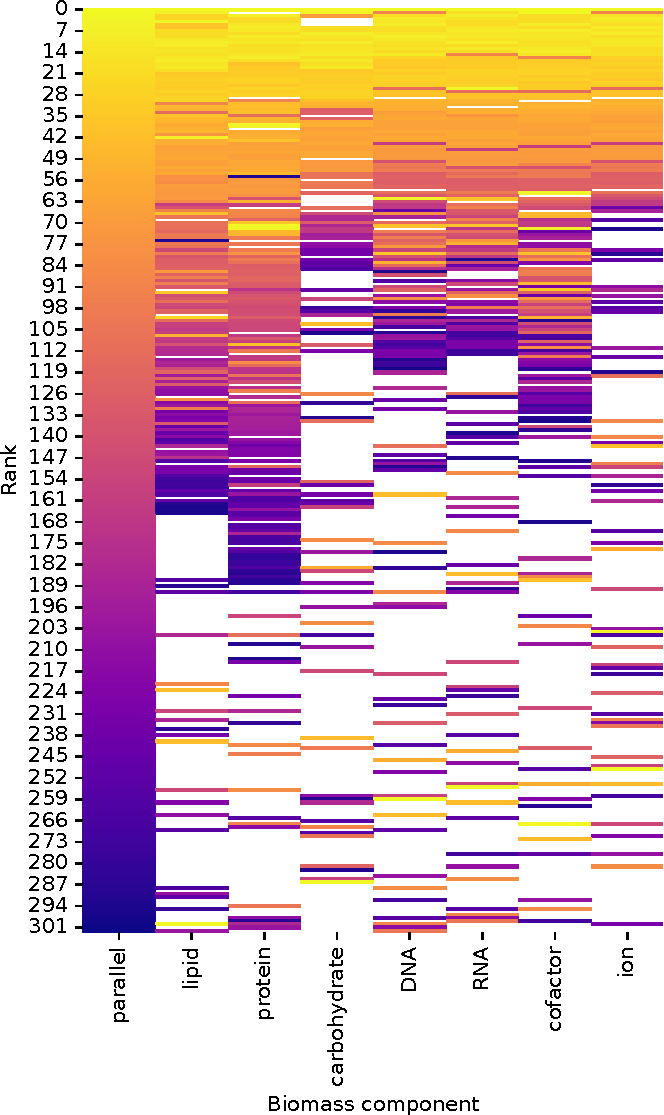
\includegraphics[width=\linewidth]{CompareEnzUse_glc01p69_pyrUnres_amm01p05_1.pdf}
    \caption{
      Rank of enzyme usage reactions in the high $\ratioabl$ case ($\exchrate{glucose}$ = \SI{1.69}{\mmolgdwh}, $\exchrate{ammonium}$ = \SI{1.05}{\mmolgdwh}).
    }
    \label{fig:model-rank-glc-highratio-rank}
  \end{subfigure}

  \begin{subfigure}[t]{0.45\textwidth}
  \centering
    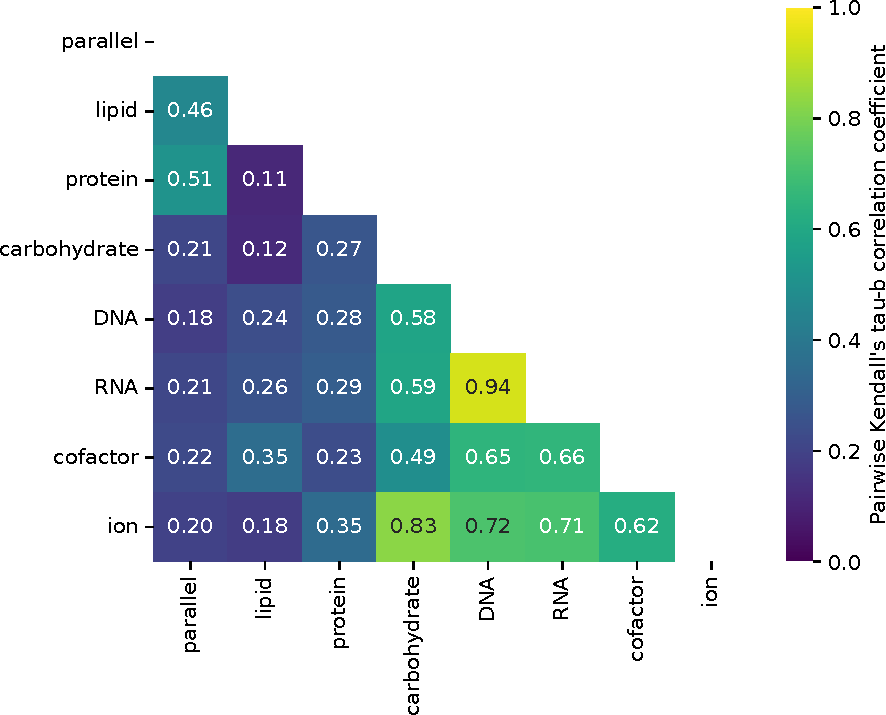
\includegraphics[width=\linewidth]{CompareEnzUse_glc16p89_pyrUnres_ammUnres_2.pdf}
    \caption{
      Pairwise Kendall's $\tau$-b rank correlation coefficients for \ref{fig:model-rank-glc-lowratio-rank}.
    }
    \label{fig:model-rank-glc-lowratio-kendall}
  \end{subfigure}%
  \begin{subfigure}[t]{0.45\textwidth}
  \centering
    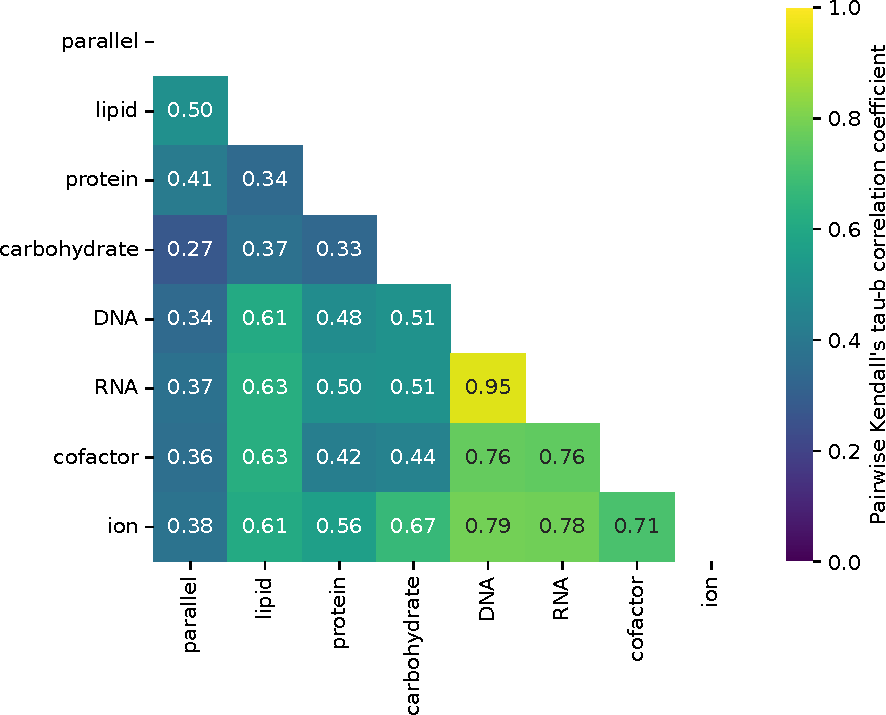
\includegraphics[width=\linewidth]{CompareEnzUse_glc01p69_pyrUnres_amm01p05_2.pdf}
    \caption{
      Pairwise Kendall's $\tau$-b rank correlation coefficients for \ref{fig:model-rank-glc-highratio-rank}.
    }
    \label{fig:model-rank-glc-highratio-kendall}
  \end{subfigure}

  \caption{
    Proteome allocation favouring sequential and parallel biosynthesis strategies, with glucose as carbon source.
    \textbf{(Top panels: \ref{fig:model-rank-glc-lowratio-rank}, \ref{fig:model-rank-glc-highratio-rank})} In the parallel case (no change to biomass equation), enzyme usage reactions are ranked, in descending order, by magnitude of flux and each assigned a colour.
    When biomass components are ablated, the ranks change, as shown by how the order of colours change from column to column.
    White indicates reactions that carry zero flux in the parallel case.
    \textbf{(Bottom panels: \ref{fig:model-rank-glc-lowratio-kendall}, \ref{fig:model-rank-glc-highratio-kendall})} Kendall's $\tau$-b rank correlation coefficient was computed for each pair of columns in the top panels to quantify the similarity between each case.
  }
  \label{fig:model-rank-glc}
\end{figure}

In both the glucose-ammonium and pyruvate-ammonium conditions, I observe that the highest $\ratioabl$ occurs at the boundary at which both the carbon source and the nitrogen source are limiting.
This leads to the hypothesis that the cell favours parallel biosynthesis of biomass components in such conditions, especially if the associated biomass components share metabolic pathways and if the conditions dictate similar levels of enzymes.

To evaluate this hypothesis, I investigated how the enzyme usage fluxes change across each round of ablation in the glucose-ammonium exchange combinations that produce the lowest and greatest $\ratioabl$ (figure~\ref{fig:model-rank-glc}), and performed the same investigation for pyruvate-ammonium exchange combinations (figure~\ref{fig:model-rank-pyr}).
As a visualisation aid, I ranked the enzyme usage reactions by magnitude of flux to emphasise how the allocation of enzymes changes in each round.
I also computed the Kendall's $\tau$-b rank correlation coefficient \parencite{kendallTREATMENTTIESRANKING1945} to quantify how similar the enzyme usage flux vectors were between each pair of rounds.

Figure~\ref{fig:model-rank-glc} suggests that in the low $\ratioabl$ condition, in which both glucose and ammonium are abundant, enzyme-available proteome allocation patterns for lipid- and protein-prioritised simulations most resemble the parallel case.
In contrast, a set of enzymes that originally had low usage fluxes in the parallel case became enzymes with the highest levels when carbohydrates, DNA, RNA, cofactors, or ions are prioritised.
This separation of biomass components into two groups according to enzyme-available proteome allocation patterns can explain how sequential biosynthesis is advantageous.
At least, the lipids and proteins can be synthesised together, followed by the other components; the order by which these two groups are synthesised can be reversed.
The high $\ratioabl$ condition, in which both glucose and ammonium are near-limiting, gives the opposite picture.
Here, allocation of the proteome to enzymes is similar across all situations, suggesting that parallel biosynthesis of biomass components may be advantageous in this situation.


\subsubsection{Pyruvate and ammonium}
\label{subsec:model-rank-pyruvate}

\begin{figure}
  \centering
  \begin{subfigure}[t]{0.45\textwidth}
  \centering
    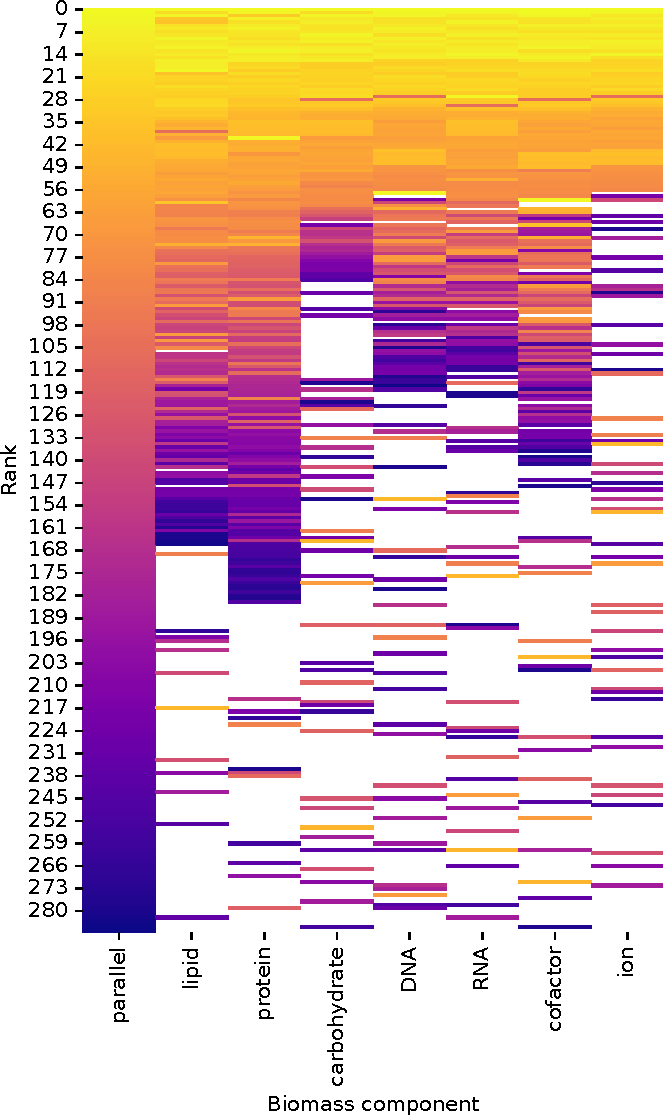
\includegraphics[width=\linewidth]{CompareEnzUse_glc00p00_pyr08p89_ammUnres_1.pdf}
    \caption{
      Rank of enzyme usage reactions in the low $\ratioabl$ case ($\exchrate{pyruvate}$ = \SI{8.89}{\mmolgdwh}).
    }
    \label{fig:model-rank-pyr-lowratio-rank}
  \end{subfigure}%
  \begin{subfigure}[t]{0.45\textwidth}
  \centering
    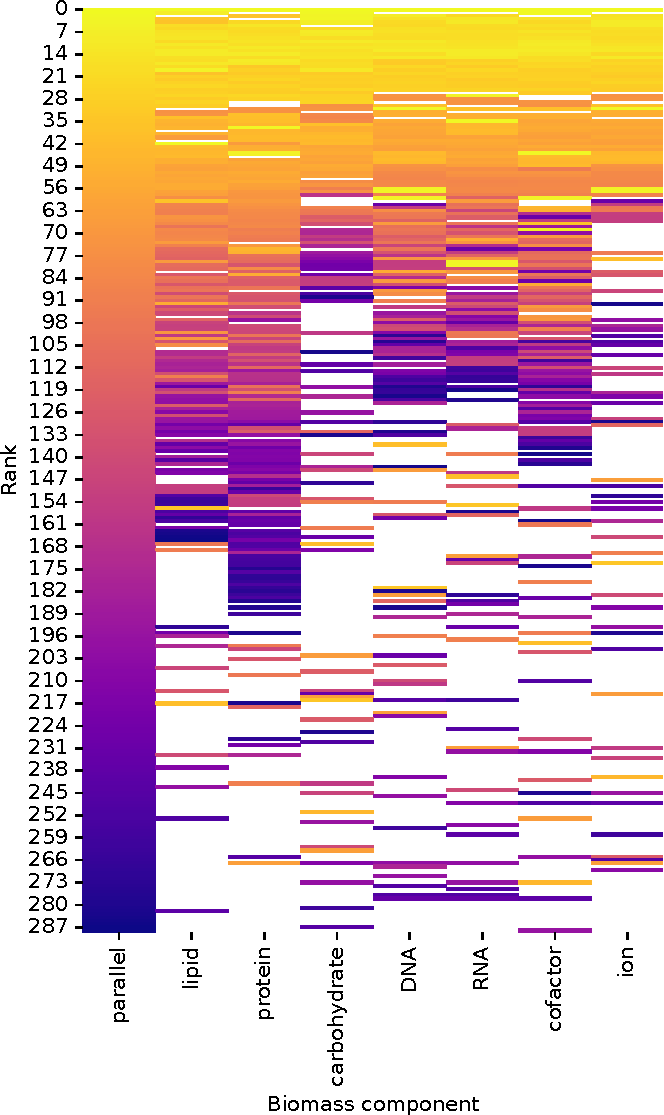
\includegraphics[width=\linewidth]{CompareEnzUse_glc00p00_pyr03p73_amm00p90_1.pdf}
    \caption{
      Rank of enzyme usage reactions in the high $\ratioabl$ case ($\exchrate{pyruvate}$ = \SI{3.73}{\mmolgdwh}, $\exchrate{ammonium}$ = \SI{0.90}{\mmolgdwh}).
    }
    \label{fig:model-rank-pyr-highratio-rank}
  \end{subfigure}

  \begin{subfigure}[t]{0.45\textwidth}
  \centering
    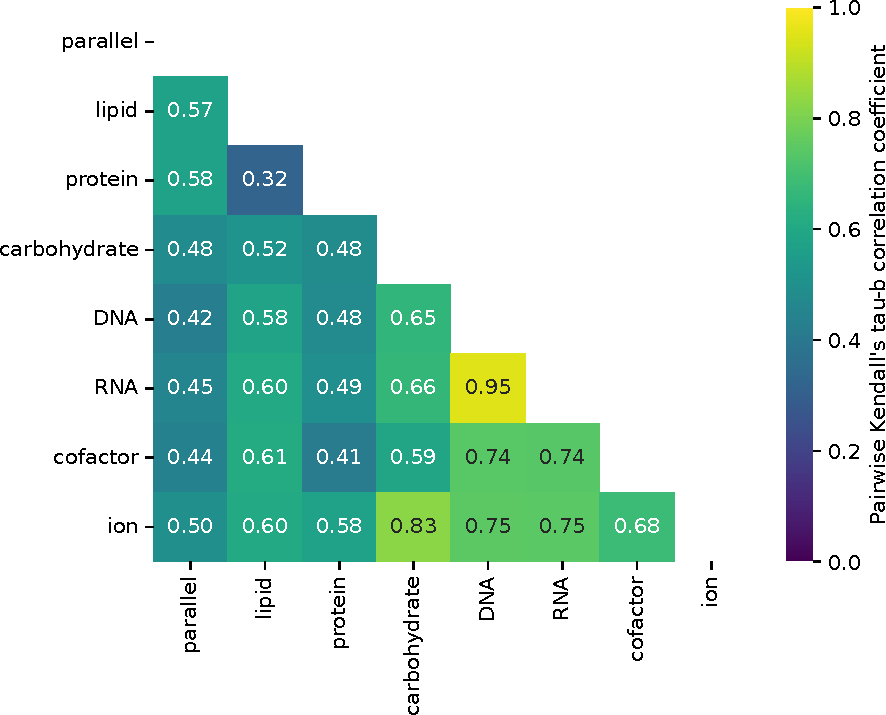
\includegraphics[width=\linewidth]{CompareEnzUse_glc00p00_pyr08p89_ammUnres_2.pdf}
    \caption{
      Pairwise Kendall's $\tau$-b rank correlation coefficients for \ref{fig:model-rank-pyr-lowratio-rank}.
    }
    \label{fig:model-rank-pyr-lowratio-kendall}
  \end{subfigure}%
  \begin{subfigure}[t]{0.45\textwidth}
  \centering
    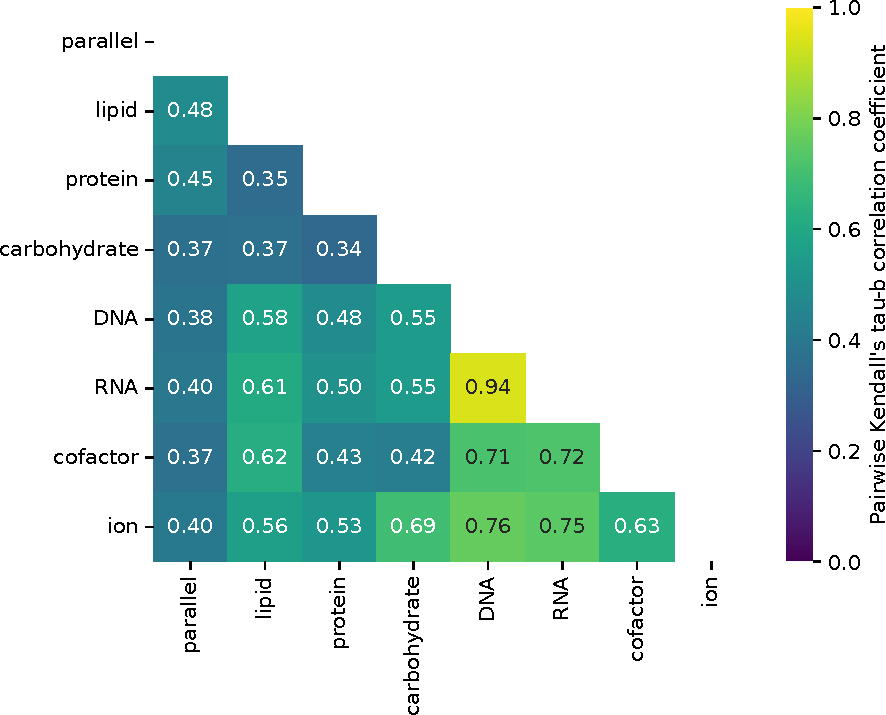
\includegraphics[width=\linewidth]{CompareEnzUse_glc00p00_pyr03p73_amm00p90_2.pdf}
    \caption{
      Pairwise Kendall's $\tau$-b rank correlation coefficients for \ref{fig:model-rank-pyr-highratio-rank}.
    }
    \label{fig:model-rank-pyr-highratio-kendall}
  \end{subfigure}

  \caption{
    Proteome allocation favouring sequential and parallel biosynthesis strategies, with pyruvate as carbon source.
    \textbf{(Top panels: \ref{fig:model-rank-pyr-lowratio-rank}, \ref{fig:model-rank-pyr-highratio-rank})} In the parallel case (no change to biomass equation), enzyme usage reactions are ranked, in descending order, by magnitude of flux and each assigned a colour.
    When biomass components are ablated, the ranks change, as shown by how the order of colours change from column to column.
    White indicates reactions that carry zero flux in the parallel case.
    \textbf{(Bottom panels: \ref{fig:model-rank-pyr-lowratio-kendall}, \ref{fig:model-rank-pyr-highratio-kendall})} Kendall's $\tau$-b rank correlation coefficient was computed for each pair of columns in the top panels to quantify the similarity between each case.
  }
  \label{fig:model-rank-pyr}
\end{figure}

However, figure~\ref{fig:model-rank-pyr} suggests that the contrast between each biomass component is lessened when pyruvate is the carbon source.

\begin{figure}
  \centering
  \begin{subfigure}[t]{0.45\textwidth}
  \centering
    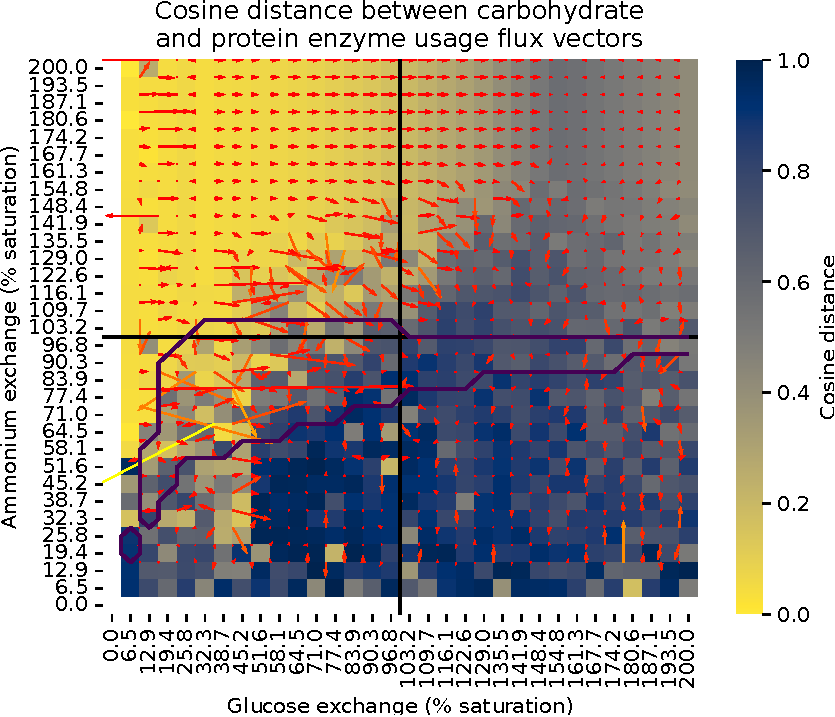
\includegraphics[width=\linewidth]{ec_grid_glc_amm_cosine}
    \caption{
    }
    \label{fig:model-noisy-glc-cosine}
  \end{subfigure}%
  \begin{subfigure}[t]{0.45\textwidth}
  \centering
    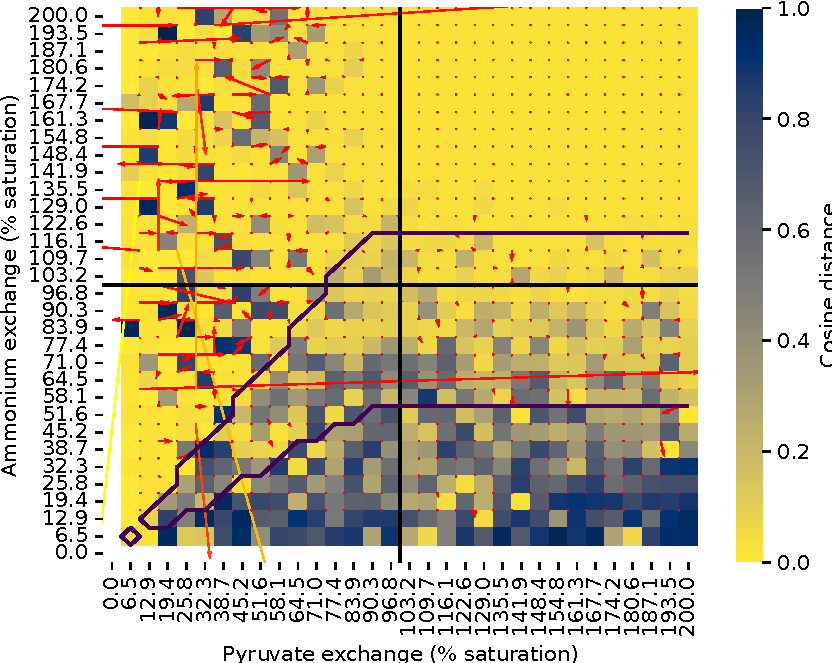
\includegraphics[width=\linewidth]{ec_grid_pyr_amm_cosine}
    \caption{
    }
    \label{fig:model-noisy-pyr-cosine}
  \end{subfigure}

  \begin{subfigure}[t]{0.45\textwidth}
  \centering
    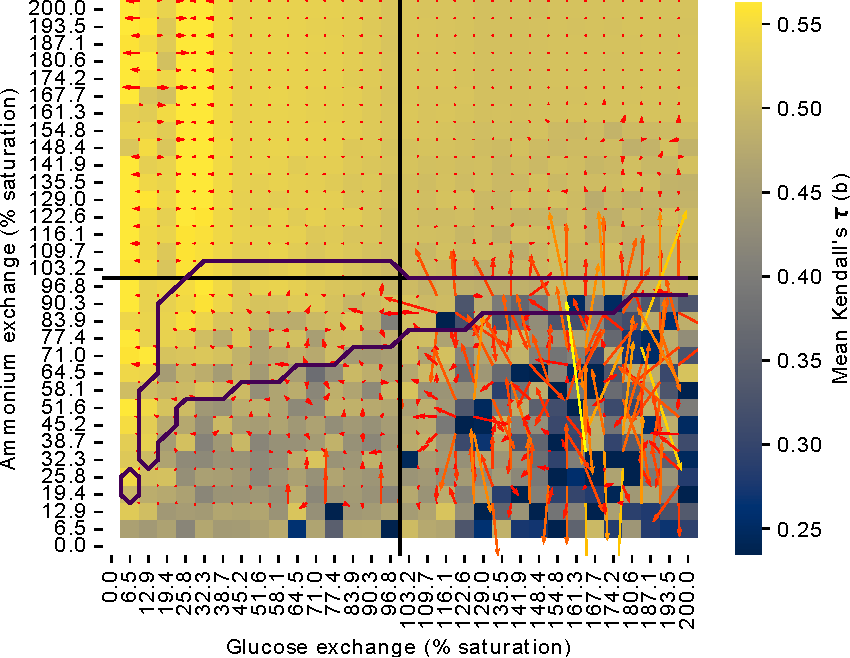
\includegraphics[width=\linewidth]{ec_grid_glc_amm_kendall}
    \caption{
    }
    \label{fig:model-noisy-glc-kendall}
  \end{subfigure}%
  \begin{subfigure}[t]{0.45\textwidth}
  \centering
    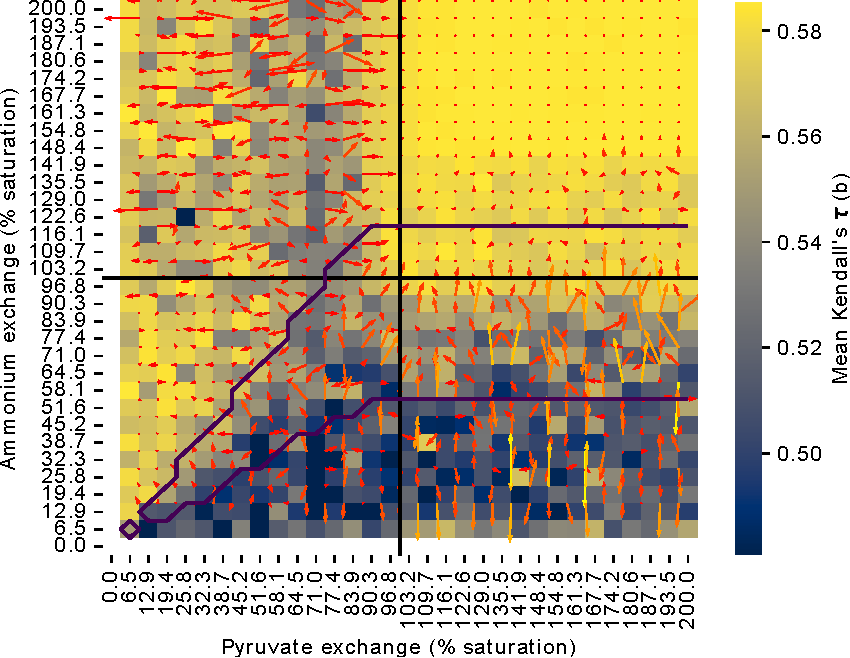
\includegraphics[width=\linewidth]{ec_grid_pyr_amm_kendall}
    \caption{
    }
    \label{fig:model-noisy-pyr-kendall}
  \end{subfigure}

  \caption{
    Measures of similarity between enzyme usage fluxes in rounds of ablation, when glucose and ammonium exchange are varied (left panels), and when pyruvate and ammonium exchange are varied (right panels).
    \textbf{(Top panels)} Cosine distance between the vector of enzyme usage fluxes when protein is prioritised and the equivalent vector when carbohydrate is prioritised, computed for all nutrient conditions.
    \textbf{(Bottom panels)} For each nutrient condition, the Kendall's $\tau$-$b$ rank correlation coefficient between the parallel case and each biomass-prioritised case was computed and the mean was found.
    Higher mean correlations suggest an advantage to parallel biosynthesis.
  }
  \label{fig:model-noisy}
\end{figure}

Upon investigation of all \num{1024} nutrient conditions in each carbon source-nitrogen source pair, it appears that the relationship between exchange rate and any measure of similarity between ablation rounds that is based on enzyme usage reactions is not continuous (figure~\ref{fig:model-noisy}).
This noise complicates drawing conclusions.
Although, in the pyruvate-ammonium case, there is a general trend that suggests that proteome allocation when carbohydrates are prioritised and when proteins are prioritised are more similar in high-pyruvate high-ammonium conditions.
There is also a trend that suggests, contrary to figure~\ref{fig:model-grid-pyr}, that parallel biosynthesis is more similar to ablated cases in high-pyruvate high-ammonium conditions, but not by a high degree.
On the contrary, in the glucose-ammonium case, there is a general trend that suggests that, at high ammonium exchange rates, increasing glucose exchange rates lead to a greater difference between the enzyme usage flux vectors when carbohydrate is prioritised and when protein is prioritised.
In all cases, there seems to be no clear relationship between the distance measures and whether $\ratioabl > 1$.

The noise in figure~\ref{fig:model-noisy} is likely explained by the multiplicity of solutions in FBA.
This phenomenon means that FBA finds the optimal value of the objective function, such as growth, but the flux vector that gives rise to this objective function may differ across each simulation or each linear optimisation solver.
This is not a problem when ablation-related quantities were computed earlier in the section because they were based on the flux of the objective function, defined as the biomass reaction, even if the biomass reaction itself was modified during ablation.
In other words, although choosing representative nutrient conditions leads to an attractive picture that may confirm the hypothesis of this section, the computational limitations of FBA may render any conclusion flawed.


\section{Conclusion}
\label{subsec:model-conclusion}

Enzyme-constrained models like GECKO are useful.
However, an appropriate method of restricting fluxes must be used, given the formalisms built in the model.

Ablation of components of the biomass reaction gives changes to enzyme allocation that are biologically relevant and also gives a way to estimate timescale of biosynthesis.
Such timescales give rise to a $\ratioabl$ ratio that can be used to assess whether sequential or parallel biosynthesis of biomass components is favoured.

A restricted proteome-available protein pool, as long as the growth rate remains realistic, makes sequential biosynthesis more advantageous.
In addition, the advantage is retained in auxotrophs and deletion strains, confirming the robustness (presence) of sequential biomass synthesis as a resource allocation strategy, and thus may explain why the metabolic cycle is still present in such strains.

Nitrogen source availability affects protein synthesis time in the sequential case, while carbon source availability affects both carbohydrate and protein synthesis times.
Both additively promote (wild type) growth rate.
These effects explain why parallel biosynthesis is advantageous when carbon and nitrogen sources are both near-limiting or when the nitrogen source is near saturation while the glucose source is over saturation.
Such patterns are dependent on the growth saturation curves on each nutrient source.

When the cell prioritises biosynthesis of each biomass component, it allocates its proteome to enzymes differently, but the allocation is similar when the cell prioritises carbohydrates, DNA, RNA, cofactors, and ions.
This could explain why parallel biosynthesis is advantageous in some conditions.
However, the multiplicity of FBA solutions complicates analysis based of fluxes.

How the cell changes its allocation of its proteome to subsystems may explain some experimental observations.
It is possible that the cell synthesises carbohydrate, DNA, and RNA around the same time so that use of  oxidative phosphorylation occur at around the same time.
This may explain cycles in dissolved oxygen concentrations.
In addition, lipid biosynthesis often requires different enzymes than the other components, and this may explain cycling of lipid stores.

The extent to which sequential biosynthesis is advantageous in different nutrient conditions and the synthesis timescales predicted may explain why yeast cells show metabolic cycles in certain nutrient conditions.
The model may provide a weak explanation of why yeast cells continue to have metabolic cycles when abruptly starved of glucose: if the glucose exchange is near zero, the ratio is less than one.
Though, a better investigation would account for switching between nutrient conditions, which the most basic forms of FBA is not built for --- it only looks at steady state, and does not `remember' past states.

The model does not account for varying protein fractions and other parameters that affect the size of $\epool$ during growth and division, and across different conditions.
For instance, \textcite{elsemmanWholecellModelingYeast2022} state that growth rate affects proteome fractions ($f$) and the saturation factor ($\sigma$)
However, because I find that $\epool$ affects the growth rate, there may be a circular relationship, and there is no guarantee that parameter values will converge if I tune the $\epool^{\prime}$ to obtain a $\gro$ that in turn affects $\epool^{\prime}$.
Furthermore, the data on biomass component fractions are old, sparse, and coarse --- as a back-of-the-envelope calculation, my investigation is perhaps sufficient.

In summary, my results show that the yeast cell may synthesise its biomass components in sequence or in parallel, subject to proteomic and nutrient availability constraints.
Although it is unrealistic to assume that synthesis of one class macromolecule excludes all others, this approach is still instructive.
It gives a back-of-the-envelope calculation to support the notion that the cell partitions biosynthesis temporally
It also gives weight to the idea that this may be one of the rationales of the existence of the yeast metabolic cycle.

% Upon closer inspection of the times and fluxes... [INSERT RESULTS AND DISCUSSION HERE]
% - How long does it take to replicate the genome?  It is biosynthesis of nucleotides + process of polymerising them.  There has to be super basic cell division cycle literature about this...
% - Fatty acids: cell may use pentose phosphate pathway and gluconeogenesis to route flow in a cycle to generate masses of NAD(P)H.  Check if the fluxes suggest this.

% <comment> Moved from end of sec:model-fba.  More appropriate as discussion re extensions to my work
However, FBA, in its most basic form, has several limitations.
It only gives a steady-state picture of metabolism, and therefore cannot be used to describe changes in fluxes over time.
Although, dynamic FBA has been developed to solve this problem \parencite{mahadevanDynamicFluxBalance2002}.
Additionally, it does not account for concentrations of metabolites.
Nevertheless, there are many derivatives of FBA to overcome these limitations and extend the method to answer additional modelling questions.
However, these derivatives are outside the scope of this thesis.
% </comment>
